\documentclass[]{usiinfbachelorproject}

\usepackage{float}
\usepackage{subcaption}
\usepackage{graphicx}
\usepackage{chngcntr}
\counterwithin{figure}{section}

\captionsetup{labelfont={bf}}

\author{Andrea Vicari}

\title{Smart--IVC}
\subtitle{Enhanced Visualization of Cities, Through Smart Visual Queries}
\versiondate{\today}
\begin{committee}
%With more than 1 advisor an error is raised...: only 1 advisor is allowed!
\advisor[Universit\`a della Svizzera Italiana, Switzerland]{Prof.}{Michele}{Lanza}
%You can comment out  these lines if you don't have any assistant
\assistant[Universit\`a della Svizzera Italiana, Switzerland]{Prof. Dr.}{Andrea}{Mocci}
\end{committee}
\newcommand{\applicationName}{Smart--IVC}

\abstract {
Web users have to aggregate different data from various sources whenever they are looking for some information on the Internet. Think about the student who is looking for a rented room near her university: she firstly uses a specific website to find the advertisement of a room for rent, she then looks for the address on another website that provides a map service to see if the house is located where she desires.\\

No such service exists that provides a unique environment in which the user can both visualize a city and interact with its elements. The only technologies available are either not exhaustive or too complex to use.\\

This thesis introduces \applicationName\ a web application that provides an intuitive interface and prevents the user from jumping from website to website. Through the form of a 3D-environment, this application provides an interactive visualisation of cities in which the user can directly “communicate” with the elements, executing queries on them. After having clicked on a building in the map, the user is able to get information (coordinates, address, floors etc.) about that construction and also find out what are the various relations between that specific building and the other entities in the city.\\

\applicationName\ is an application accessible by everyone and that aims to enhance the city visualisation, getting closer to the user needs.
}

\begin{document}
\maketitle
\thispagestyle{empty}
\tableofcontents
\newpage
\thispagestyle{empty}
\listoffigures
%\listoftables
\newpage
%%%%%%%%%%%%%%%%%%%%%%%%%
%%%%%%%%%%%%%%%%%%%%%%%%%
\section{Introduction} \label{introduction}
%%%%%%%%%%%%%%%%%%%%%%%%%
Cities nowadays are in constant evolution. They change their structure over time through the appearance of new entities and the disappearance of old ones, thus they are very unsteady and prone to changes. Important changes might be considered with regard to the deployment and management of all types of infrastructures within cities. For example, the decision of which building to demolish in order to make space for the construction of a new mall in a city.\\

Moreover, cities have a very large impact on the economic and social development of nations: they represent the real foundation where people live, where companies have their business and in which numerous services are provided. Often, a city overview is not available, so decision may be taken without having a big picture of the surrounding environment. This could lead to choices that might have a negative impact on the current city, reducing the efficiency and the life quality of the citizens. Also, data is not very well aggregated since different information about the same city can be provided by different public and online services for example Google and OpenStreetMap or by public city entities like the cadastre office.\\

To control these changes and to aggregate this data, a visualization, which provides a city overview, is required. Such a visualization is considered to be the first step towards what it is called a Smart City. A Smart City can be defined as a city which uses information and communication technologies so that its critical infrastructure as well as its components and public services provided are more interactive, efficient and so that citizens can be made more aware of them.\\

\subsection{Contributions}
\applicationName\ aims to solve the problem generated by the static and non--aggregated nature of data regarding cities (as mentioned above) through an Interactive 3D--Visualization model. Therefore, the main contributions that \applicationName\ provides are:
\begin{itemize}
	\item The visualization of a 3D city model. As a use case for this Bachelor Project, the city of Lugano has been taken into account.
	\item The interactivity that the user has with the entities inside the city: buildings can be clicked in order to receive information about them and in order to receive information between the selected building itself and the rest of the entities in the city.
	\item The possibility to have a graphical city overview using a very intuitive system of visual queries which produce results that are immediately visible through the highlighting or colouring of the buildings. 
\end{itemize} 
\subsection{Structure of the report}
\begin{itemize}
	\item {\bf Chapter 2} discusses the state of the art. It talks about already existing tools which allow city visualization in a virtual environment. In particular, it focuses on tools that use the Cesium framework comparing and contrasting the existing features with the ones proposed in \applicationName.
	\item {\bf Chapter 3} is the main chapter of the entire report. It shows how \applicationName\ has been developed step by step. The decisions that have been taken and the technologies adopted will be explained and discussed in detail starting from the parsing of the unique .xml file provided by the Comune of Lugano and ending with the final result (i.e., the 3D--visualization of the entire city). 
	\item {\bf Chapter 4} illustrates showing some use cases of the application. Examples will be illustrated and explained in detail, in order to show the features proposed by \applicationName. 
	\item {\bf Chapter 5} is the conclusion of this report. Here, the current limitations of the application will be presented. Finally, we will discuss and analyze the future work and the different paths that \applicationName\ might take.
\end{itemize}
%%%%%%%%%%%%%%%%%%%%%%%%%
%%%%%%%%%%%%%%%%%%%%%%%%%
\section{State of the Art} \label{stateOfTheArt}
%%%%%%%%%%%%%%%%%%%%%%%%%
City visualization is a subject undergoing intense study, therefore it is easy to find new projects about it everyday, on the Internet. Still, the uniqueness of \applicationName\ resides on the fact that it provides not only a visualization of a city but, above all, it gives the user the possibility to interact with the city itself through a simple system of visual queries.\\

Before getting into the details with \applicationName, we will clarify the current state of city visualization and, since the projects about this topic are so various and so many, in this Chapter, we will present the ones that relate most with the final outcome of this Bachelor Project.\\

At first, we will present some 3D--city--model based on OpenStreetMap data, as {\bf OSMBuildings}, {\bf F4 Map} and {\bf ViziCities}. Then, we will introduce the {\bf Cesium framework}, since it has been used used as a basis for \applicationName. At the end, we will analyze the work done by the {\bf Swiss Geospatial Portal} (still using Cesium), in order to compare it with the application described in this report. 
\subsection{OpenStreetMap--Based Frameworks}
OpenStreetMap\footnote{OpenStreetMap: phttp://www.openstreetmap.org/} is a project that creates and distributes free geographic data for the world. During the last decade, the third dimension has become a growing topic at OSM, so it is now possible to add detailed buildings and a lot of minor objects. Here, some of the frameworks that use this data, will be analyzed.
\subsubsection{OSMBuildings}
OSMBuildings\footnote{OSMBuildings: https://osmbuildings.org/} is an engine for displaying 3D buildings on a web map. It uses information on buildings provided by OpenStreetMap and it renders them on a map layer.\\Altough in some cases, buildings are very detailed (e.g., in big cities like New York or Berlin), it does only provide a visualization without any kind of interaction.
\begin{figure} [H]
\centering
\includegraphics[width=0.8\textwidth]{chapter2/images/OSM_Building}
\caption{A visualization of New York city using OSMBuildings}
\label{fig:OSM_Building}
\end{figure}

\subsubsection{F4 Map}
The F4 Map\footnote{F4 Map: http://demo.f4map.com/} is an OSM-based 3D map using the WebGL technology. Also this map, uses Open Street Map's buildings but also adds some non--OSM--provided features like trees, cranes and other data.\\
 Some 3D models are used (not based on buildings data in OpenStreetMap) for some specific buildings (e.g. the Eiffel Tower in the example below).
\begin{figure}[H]
\centering
\includegraphics[width=0.8\textwidth]{chapter2/images/F4-Map}
\caption{A visualization of Paris using F4 Map}
\label{fig:F4-Map}
\end{figure}
Unfortunately, the F4 group does not provide any kind of documentation and this project is not open source.
\subsubsection{ViziCities}
The third and last map that uses OSM information about buildings is ViziCities\footnote{ViziCities: https://github.com/UDST/vizicities} , a framework for 3D geospatial visualization in the browser. Its code is available on GitHub since it is an OpenSource project but they are still at version 0.3 of the application.\\It lets the developer to add some useful information to the map like routes and GeoJSON (i.e., a format for encoding a variety of geographic data structures) but is still very limited and not very prone to interactivity.
\begin{figure}[H]
\centering
\includegraphics[width=0.8\textwidth]{chapter2/images/vizicities-Map}
\caption{A visualization of New York city using ViziCities}
\label{fig:vizicities-Map}
\end{figure}

\subsection{Cesium}
\begin{figure} [H]
\centering

\includegraphics[width=0.8\textwidth]{chapter2/images/cesium_logo}
\caption{Cesium logo and Cesium Virtual Globe}
\label{fig:cesium_logo}
\end{figure}
Cesium\footnote{Cesium: https://cesiumjs.org/} is an open-source JavaScript library for world-class 3D globes and maps that is used to create a web-based globe and map for visualizing dynamic data. This framework runs using WebGL, a JavaScript API for rendering 3D graphics within any compatible web browser that allows GPU--accelerated usage of physics and image processing and effects as part of the web page canvas.\\ 
The features that Cesium provides are the following:
\begin{itemize}
	\item {\bf A virtual globe:} a three-dimensional software model or representation of the Earth that provides the user with the ability to freely move around in the virtual environment by changing the viewing angle and position.
	\item {\bf Different imagery providers:} it allows to draw and layer on high-resolution imagery (maps) from several standard services directly on the virtual globe. 
	\begin{figure} [h]
		\centering
		\begin{subfigure}[b]{0.3\textwidth}
			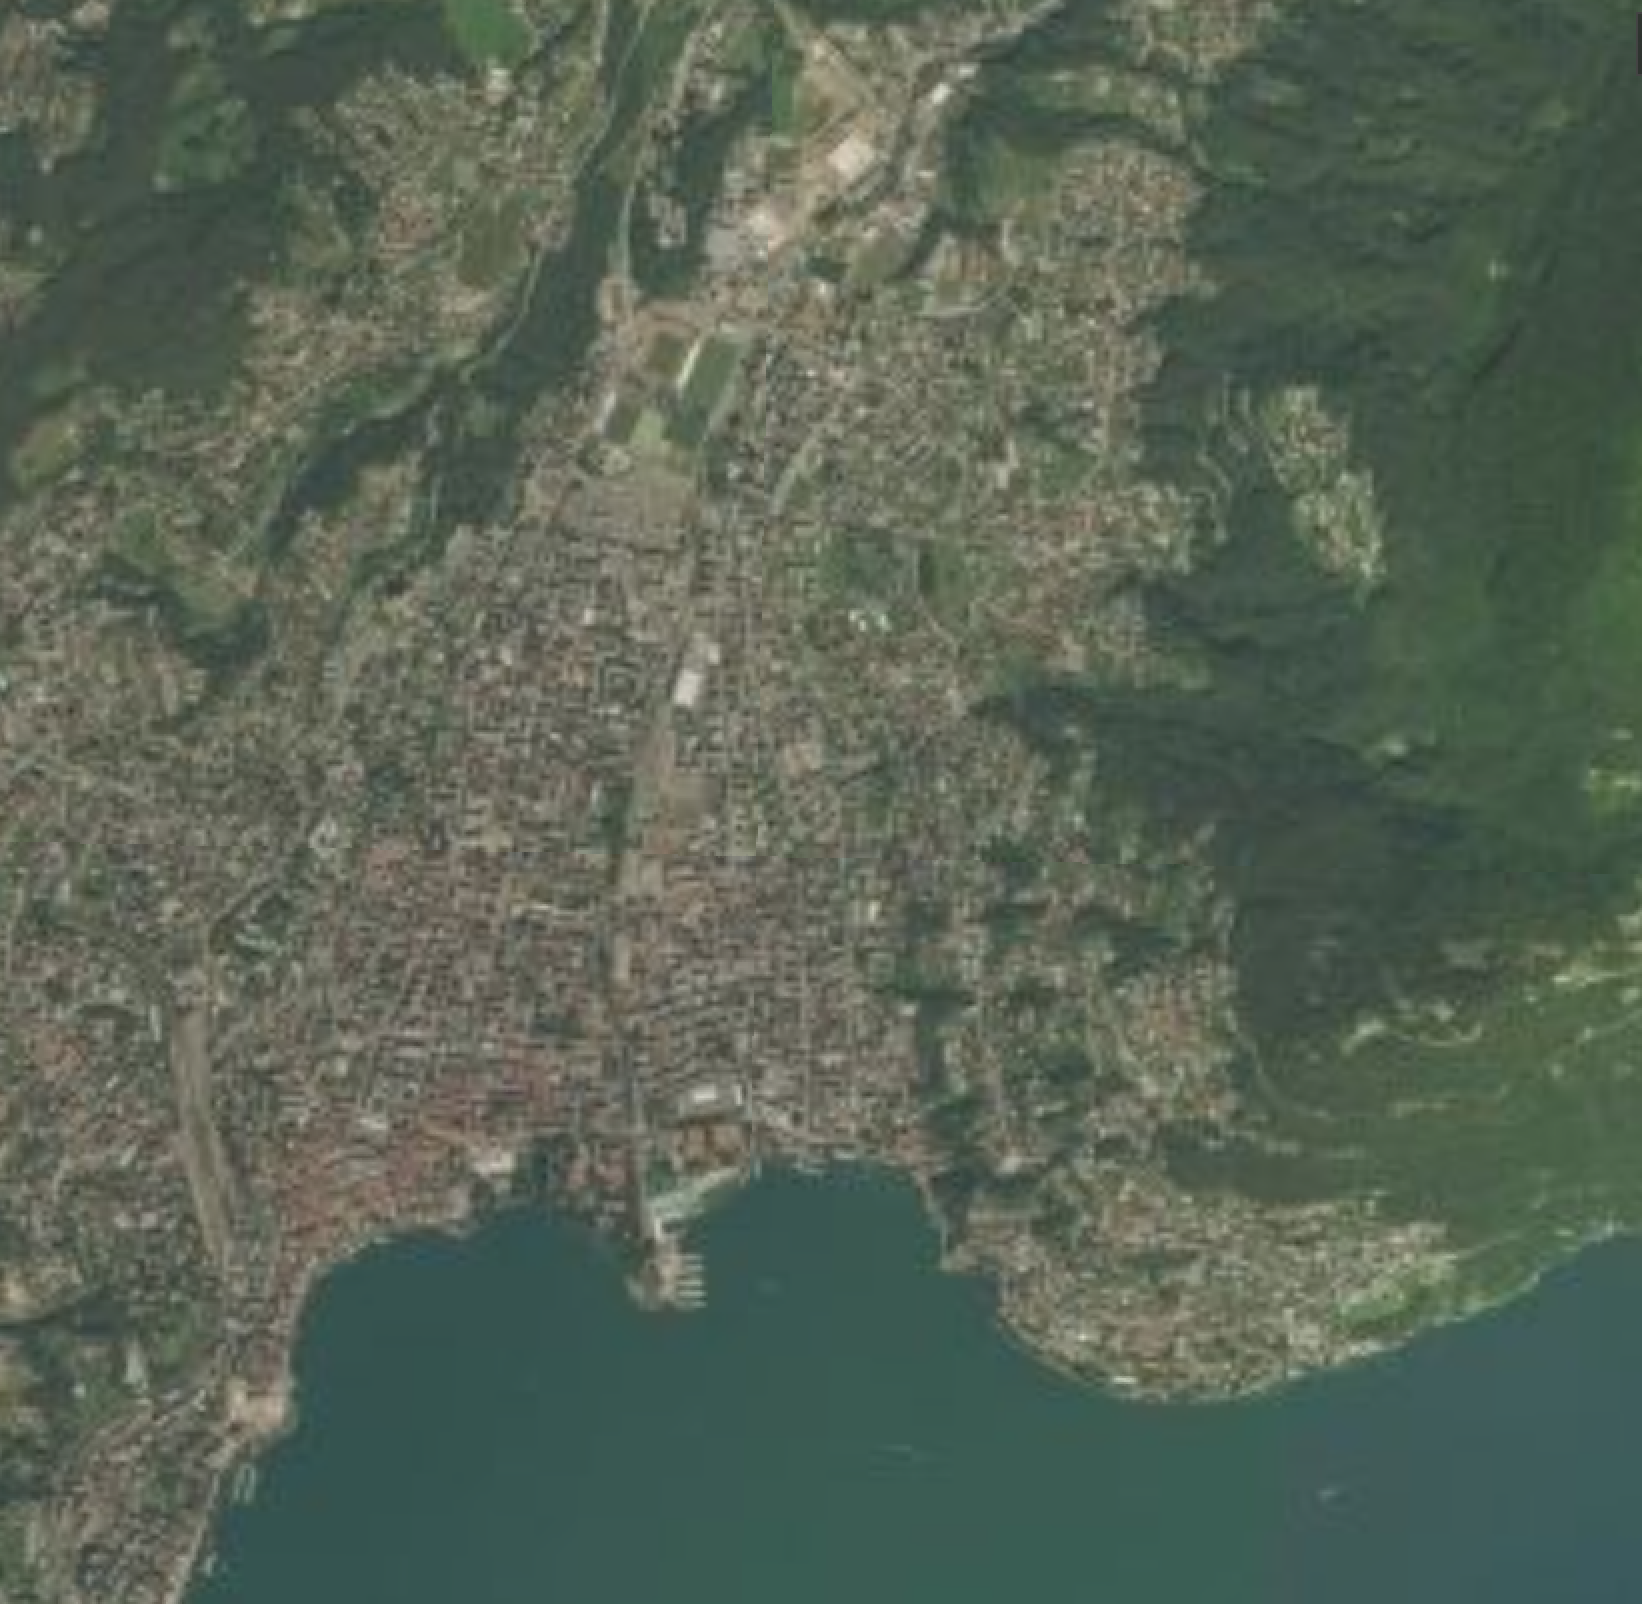
\includegraphics[width=1\textwidth]{chapter2/images/Bing-Map}
			\caption{High-resolution, mesh-based terrain provided by Bing}
			\label{fig:Bing-Map}
		\end{subfigure}
		 \qquad
		\begin{subfigure}[b]{0.3\textwidth}
			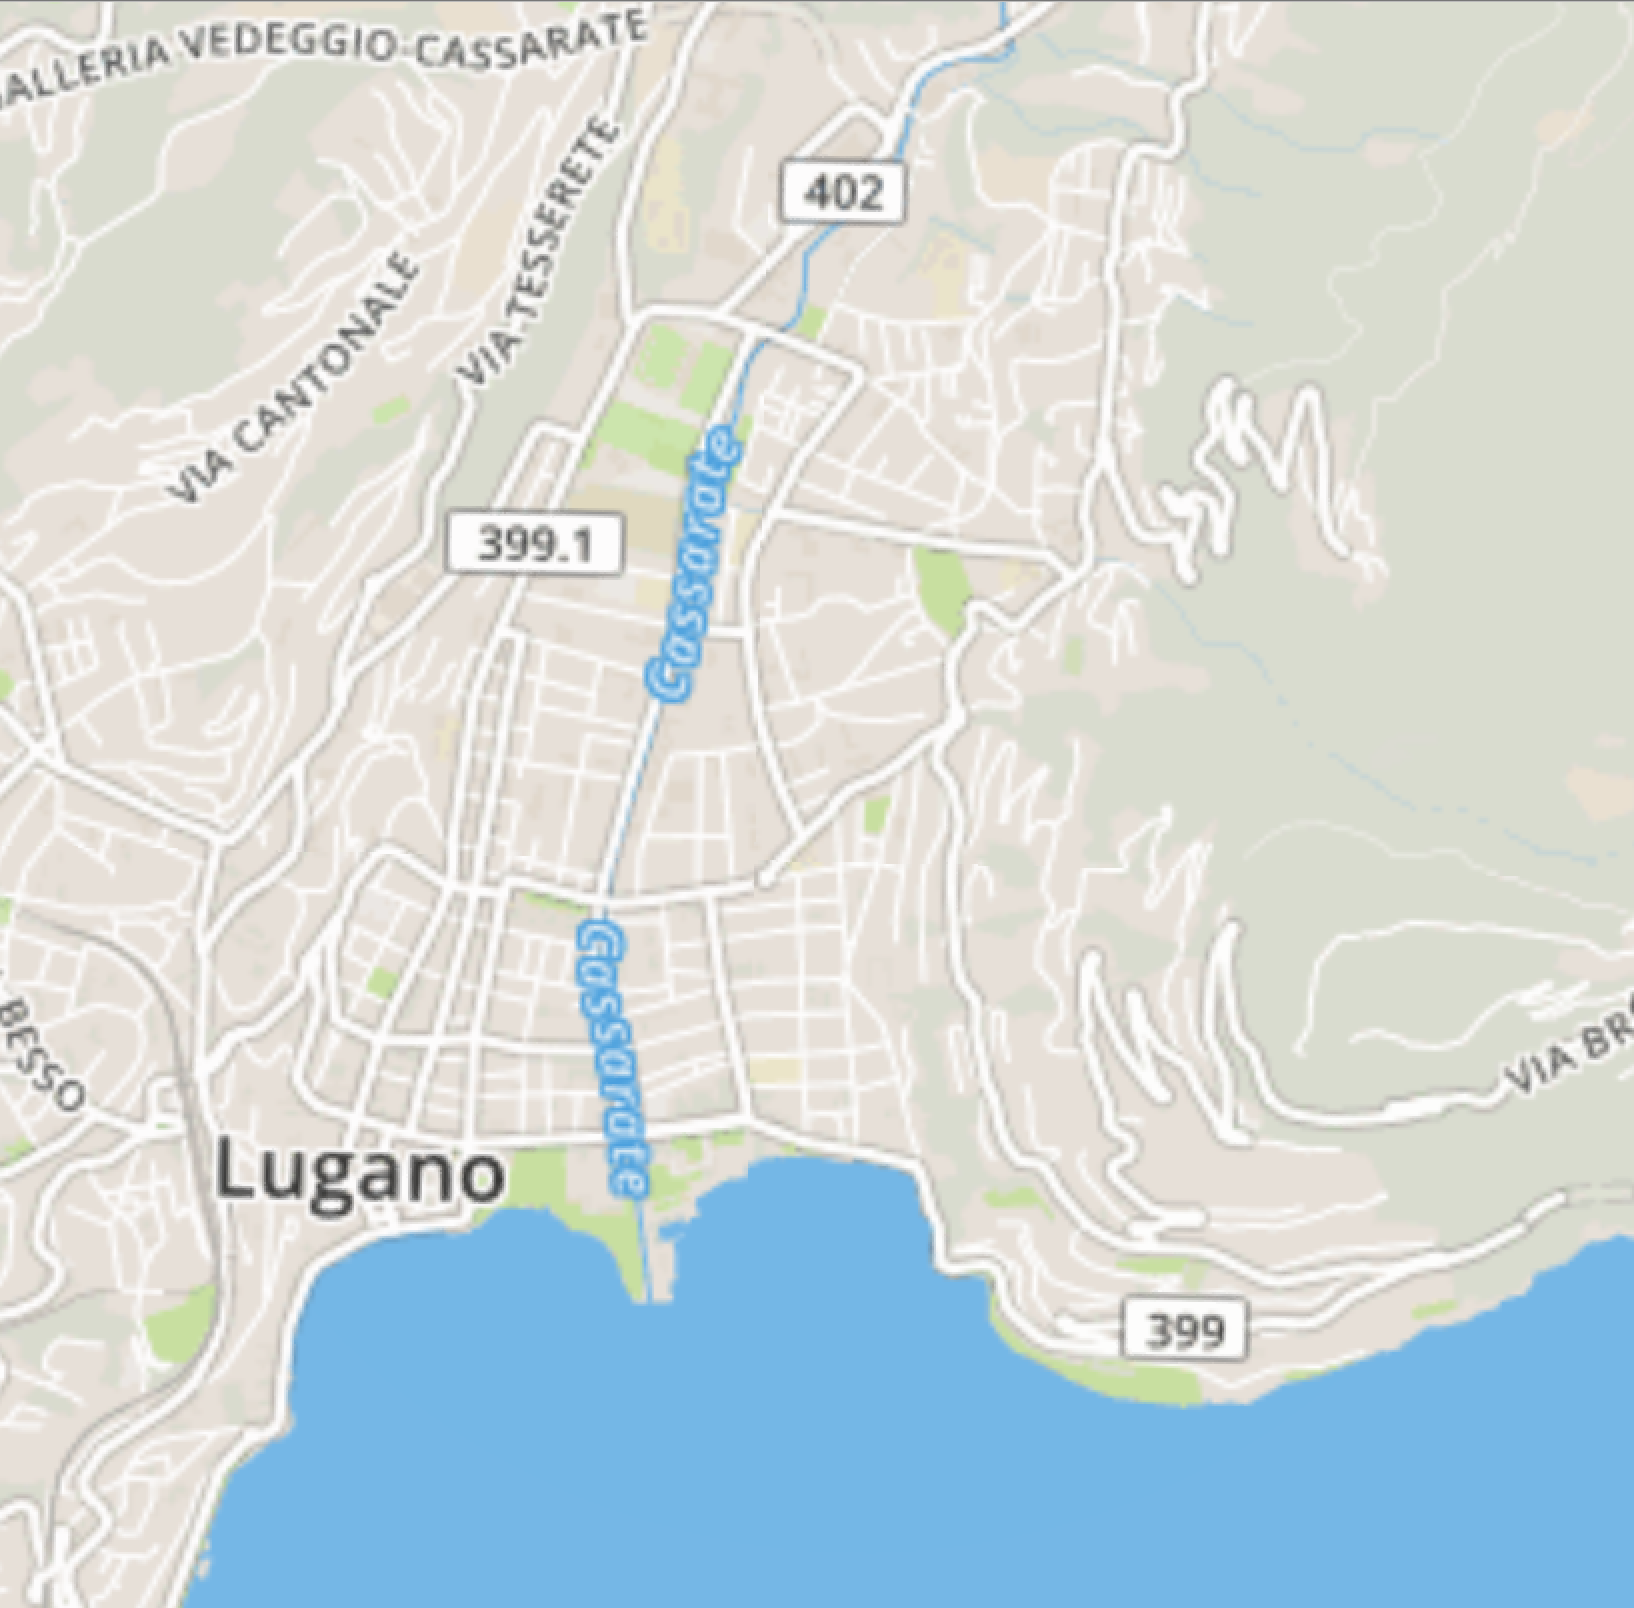
\includegraphics[width=0.993\textwidth]{chapter2/images/Mapbox-Map}
			\caption{Streets basic imagery provided by Mapbox}
			\label{fig:Mapbox-Map}
		\end{subfigure}
		\caption{Example of two imagery providers available on Cesium}
	\end{figure}

	\item {\bf Different terrain providers:} it allows to visualize global high-resolution terrains and water effects for oceans, lakes, and rivers, but mainly the possibility to represent mountain peaks, valleys, and other terrain features. 
	\begin{figure} [H]
		\centering
		\begin{subfigure}[b]{0.3\textwidth}
			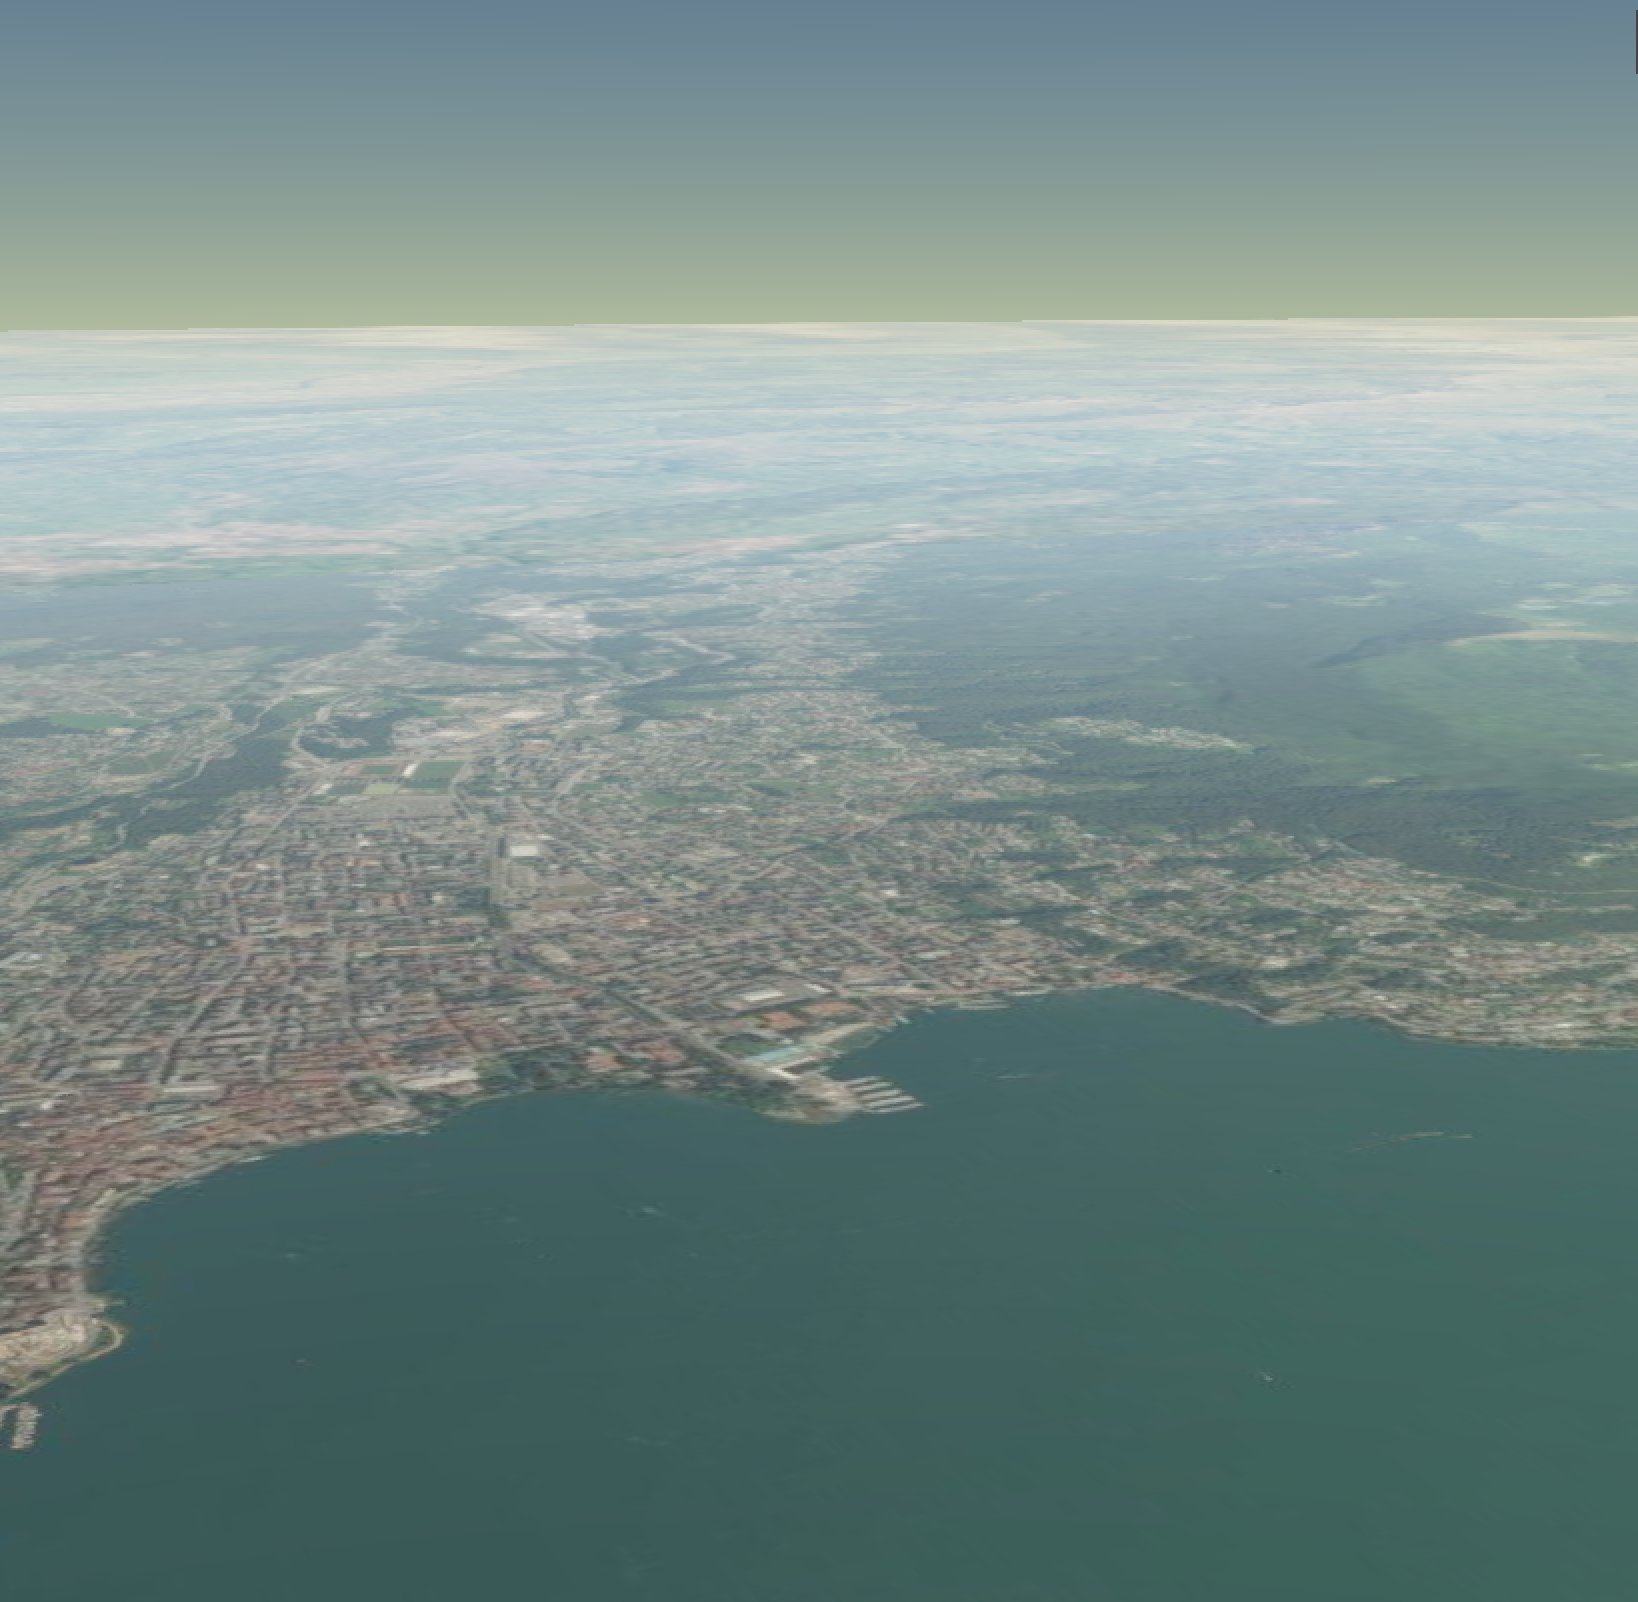
\includegraphics[width=1\textwidth]{chapter2/images/2D-Map}
			\caption{The standard WGS84 Ellipsoid}
			\label{fig:2D-Map}
		\end{subfigure}
		 \qquad
		\begin{subfigure}[b]{0.3\textwidth}
			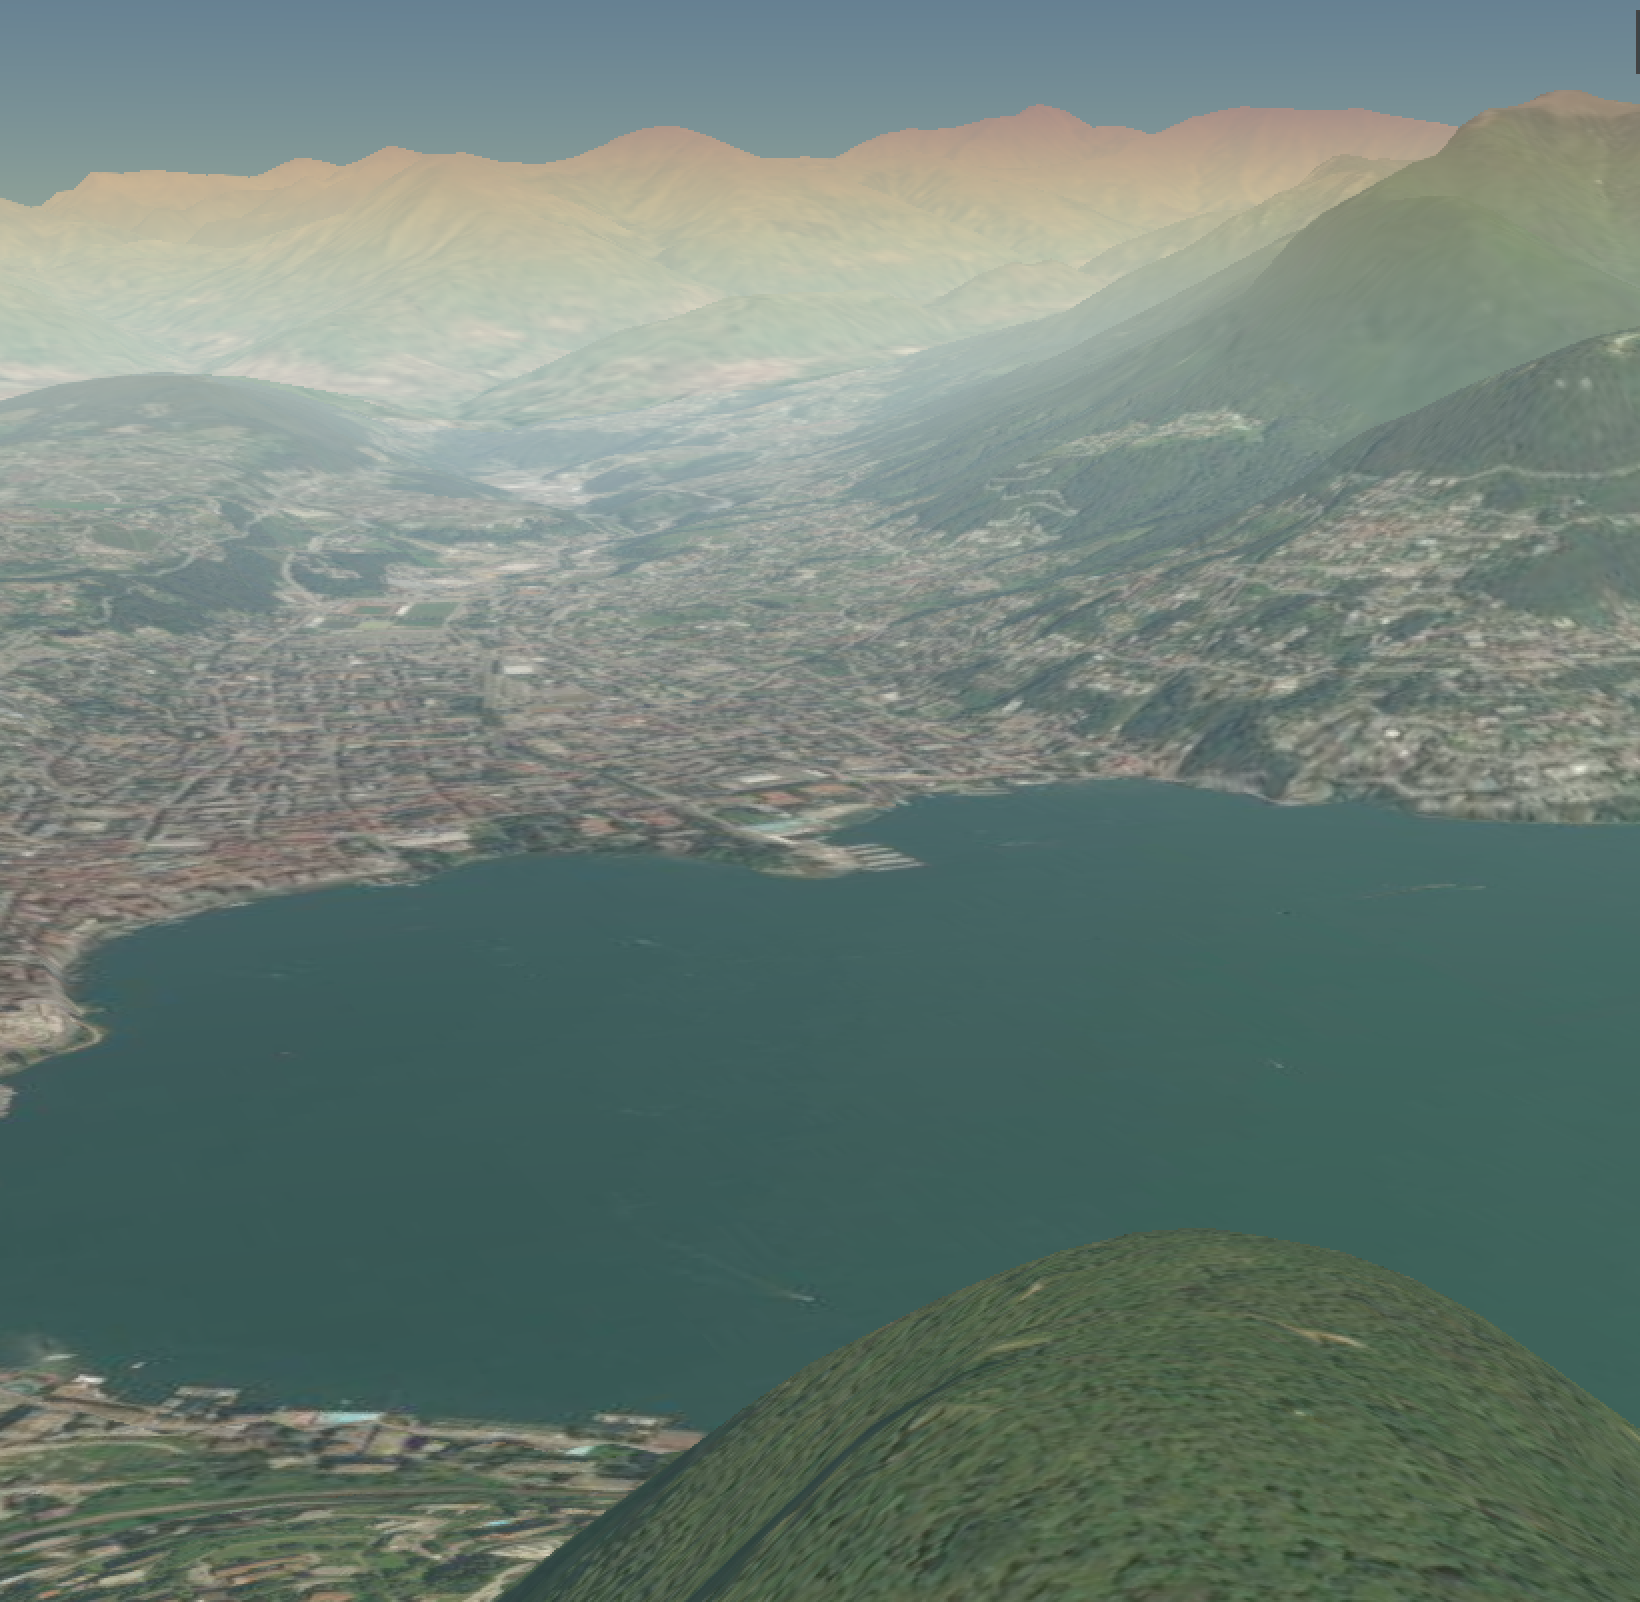
\includegraphics[width=0.993\textwidth]{chapter2/images/3D-Map}
			\caption{Terrain meshes provided by STK}
			\label{fig:3D-Map}
		\end{subfigure}
		\caption{Example of two terrain providers available on Cesium, this shows the benefits of a 3D globe compared to a 2D map.}
	\end{figure}
	\item {\bf Huge number of APIs provided:} since the uses of Cesium are really various, Cesium provides a very high number of APIs in order to control every aspect of the web application, i.e., draw every kind of geometry, handle animations, etc\dots\\The official website of Cesium also provides a complete documentation, various examples, and playgrounds.
\end{itemize} 
\subsubsection{Cesium: 3D-Tiles}
Cesium's repository on GitHub\footnote{Cesium GitHub Repository: https://github.com/AnalyticalGraphicsInc/cesium} has an open fork called ``3D-Tiles''\footnote{Cesium 3D-Tiles Fork: https://github.com/AnalyticalGraphicsInc/3d-tiles}. As specified by the contributors of this fork:  ``In 3D Tiles, a tileset is a set of tiles organized in a spatial data structure, the tree. Each tile has a bounding volume completely enclosing its contents. The tree has spatial coherence; the content for child tiles are completely inside the parent's bounding volume. To allow flexibility, the tree can be any spatial data structure with spatial coherence, including k-d trees, quadtrees, octrees, and grids.''
\begin{figure} [H]
\centering
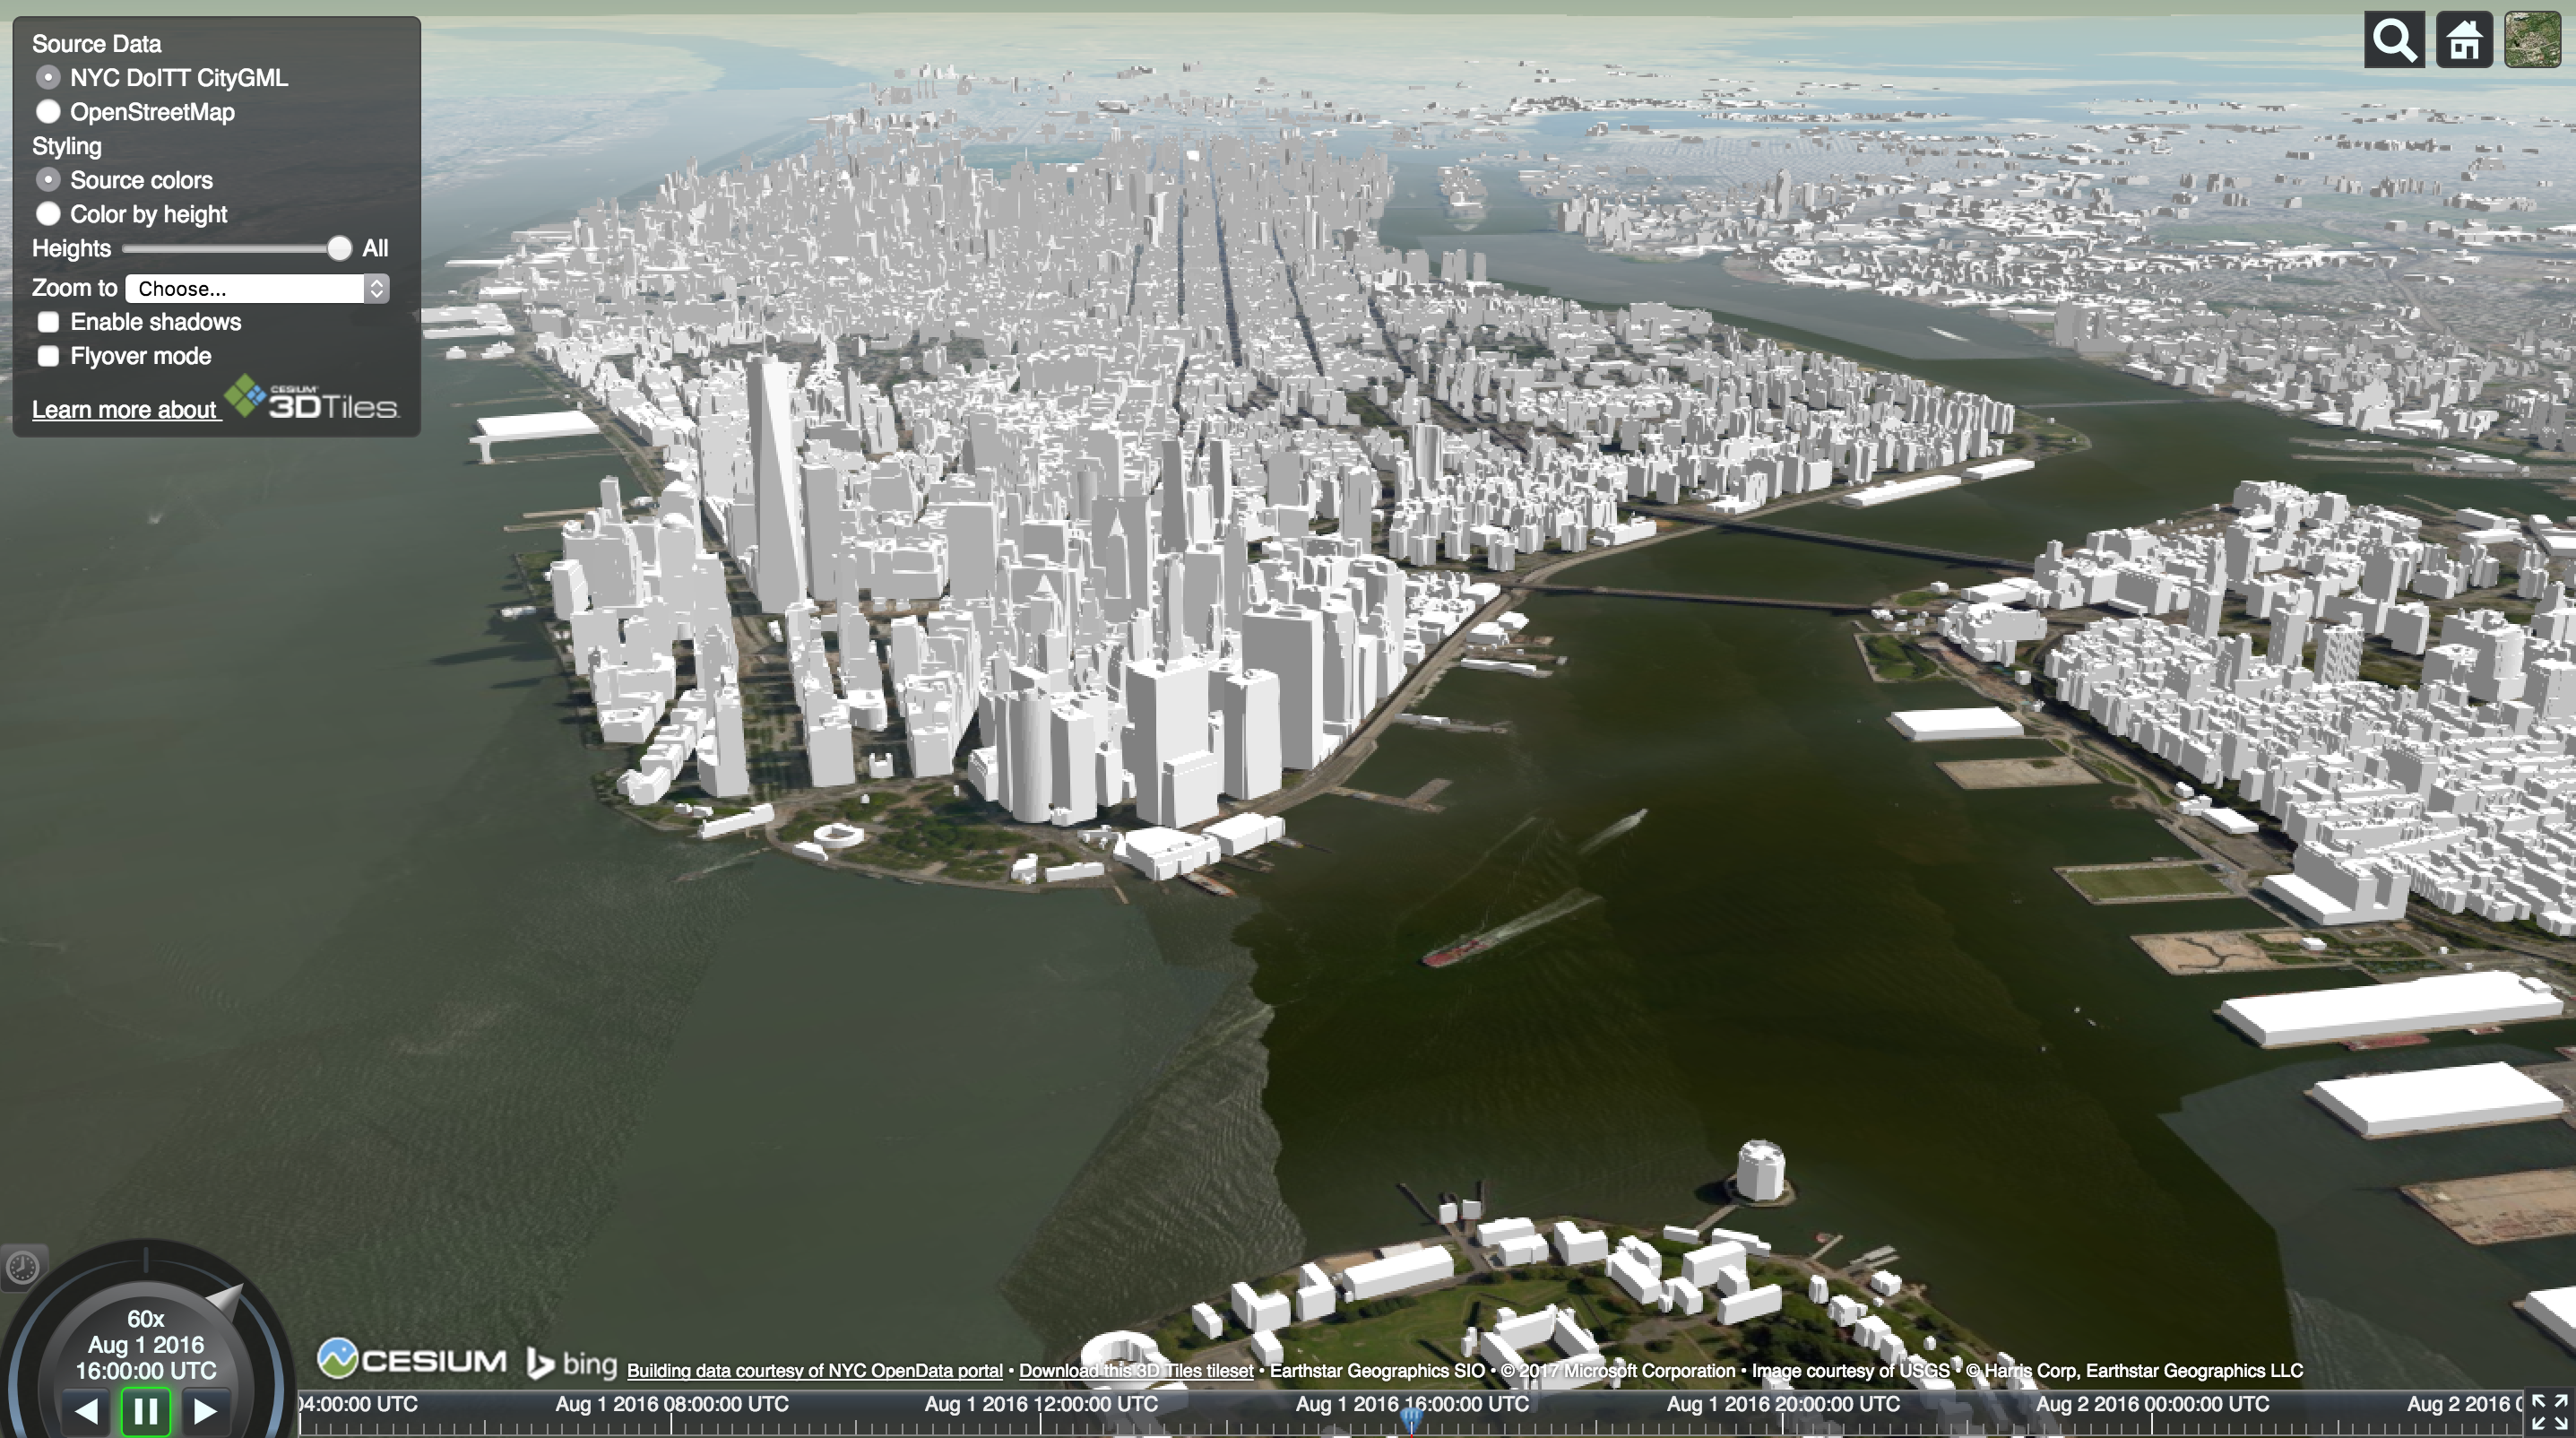
\includegraphics[width=0.8\textwidth]{chapter2/images/NewYorkCityCesium3dTiles}
\caption{An example showing a 3D visualization of the city of New York. Using Cesium 3D Tiles Tecnhology}
\label{fig:NewYorkCityCesium3dTiles}
\end{figure}
Unfortunately, being Cesium 3D--Tiles still under development, it is not provided any kind of documentation about it. Still, in a recent post on Cesium Forum, it is possible to understand that Cesium 3D--tiles fork will be soon merged to the main branch and therefore, also a complete documentation will be provided. \\In the meantime, Cesium 3D--Tiles developers are available to help programmers interested in using this technology using their forum\footnote{Developers' help forum: http://tiny.cc/884tly}.

\subsubsection{Swiss Geospatial Portal Using 3D Tiles}
Swisstopo, the Swiss Federal Geoportal is a federal government platform that facilitates public access to Swiss spatial data.
This agency produces detailed maps of Switzerland and also documents geological, geodesic, and topographical changes in the landscape.\\
Swisstopo is one of the pioneers in implementing 3D Tiles to process its extensive data collection and Cesium to visualize it. The beta visualization of their 3D Geoportal is available, it makes their national geodata collection widely available\footnote{Swisstopo implementing 3D--Tiles: http://tiny.cc/0s5tly}.
\begin{figure} [H]
\centering
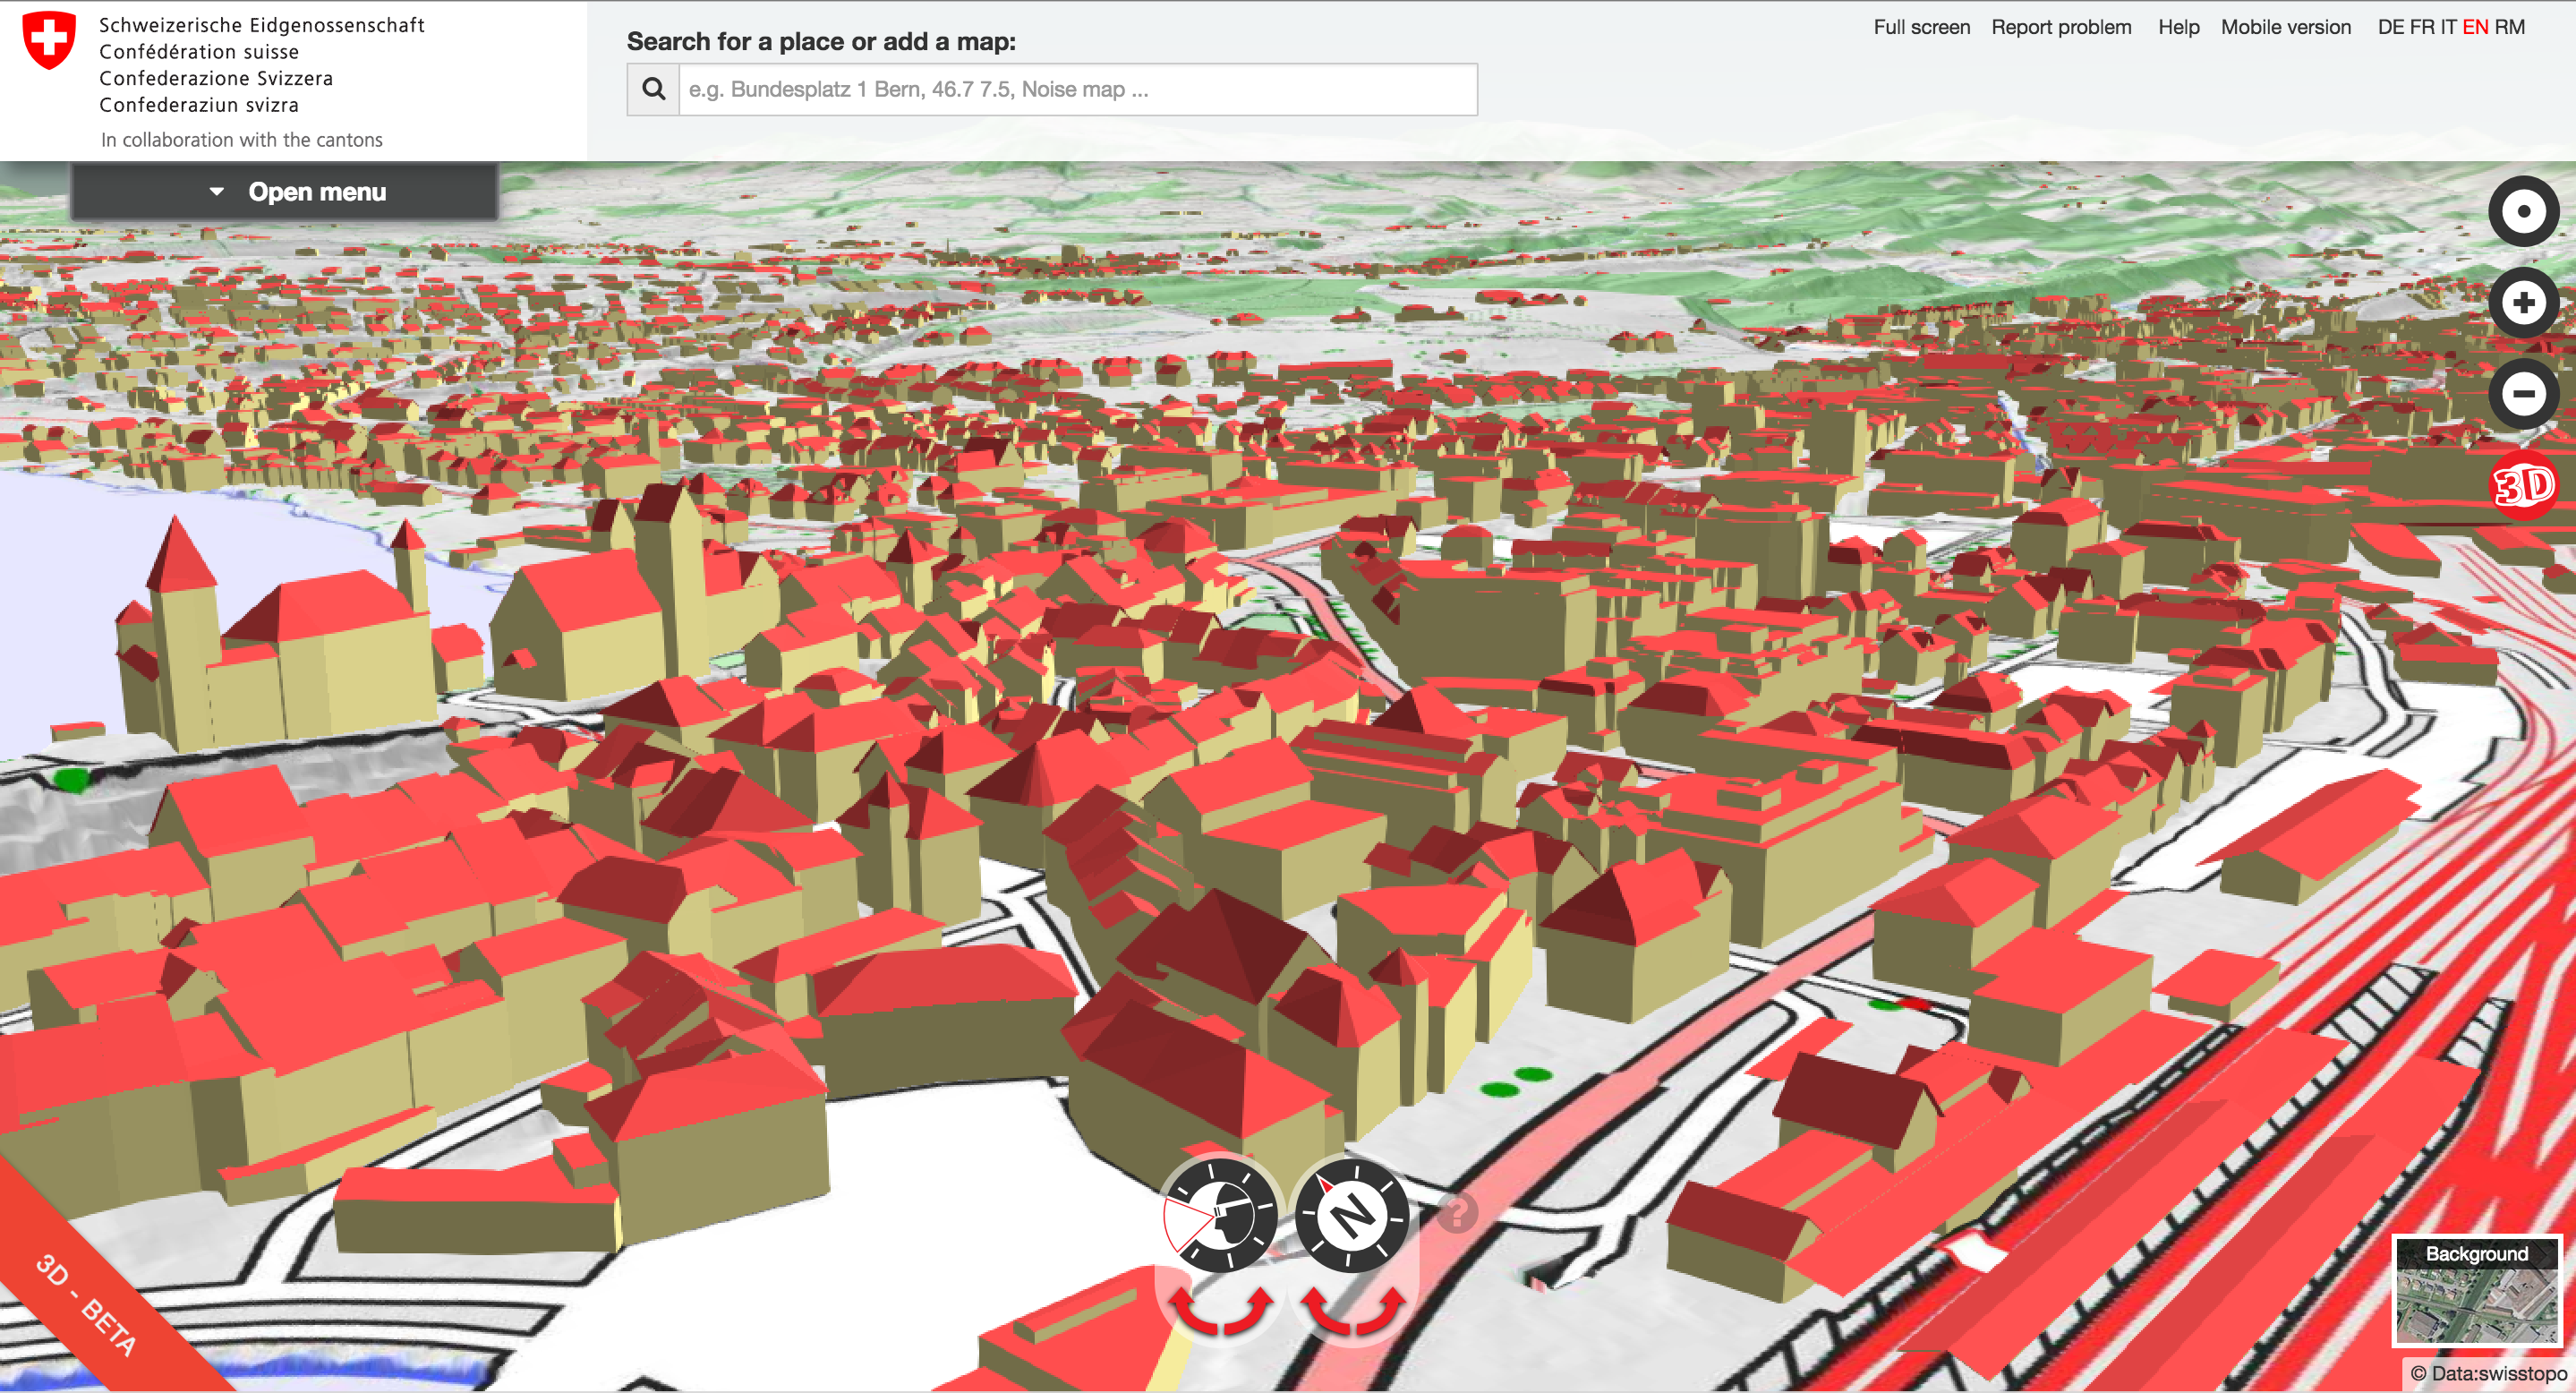
\includegraphics[width=0.8\textwidth]{chapter2/images/BernCitySwissTopo}
\caption{A 3D visualization of the city of Bern in the Swiss Geospatial Portal. Using Cesium 3D Tiles Tecnhology}
\label{fig:BernCitySwissTopo}
\end{figure}
The work done by Swisstopo, so far, consists in placing the 3D--models of buildings in some of the cities in the norther part of Switzerland (e.g., Bern, Rapperswil-Jona, Winterthur, etc\dots ). It is not provided any kind of interaction with the buildings.\\
Swisstopo provides a service in which it is possible to buy the 3D--models of the buildings, they are not highly detailed but they contain important information about the shape of the roof as can be seen in Figure\ref{fig:swisstopoBuildingModel}.
\begin{figure} [H]
\centering
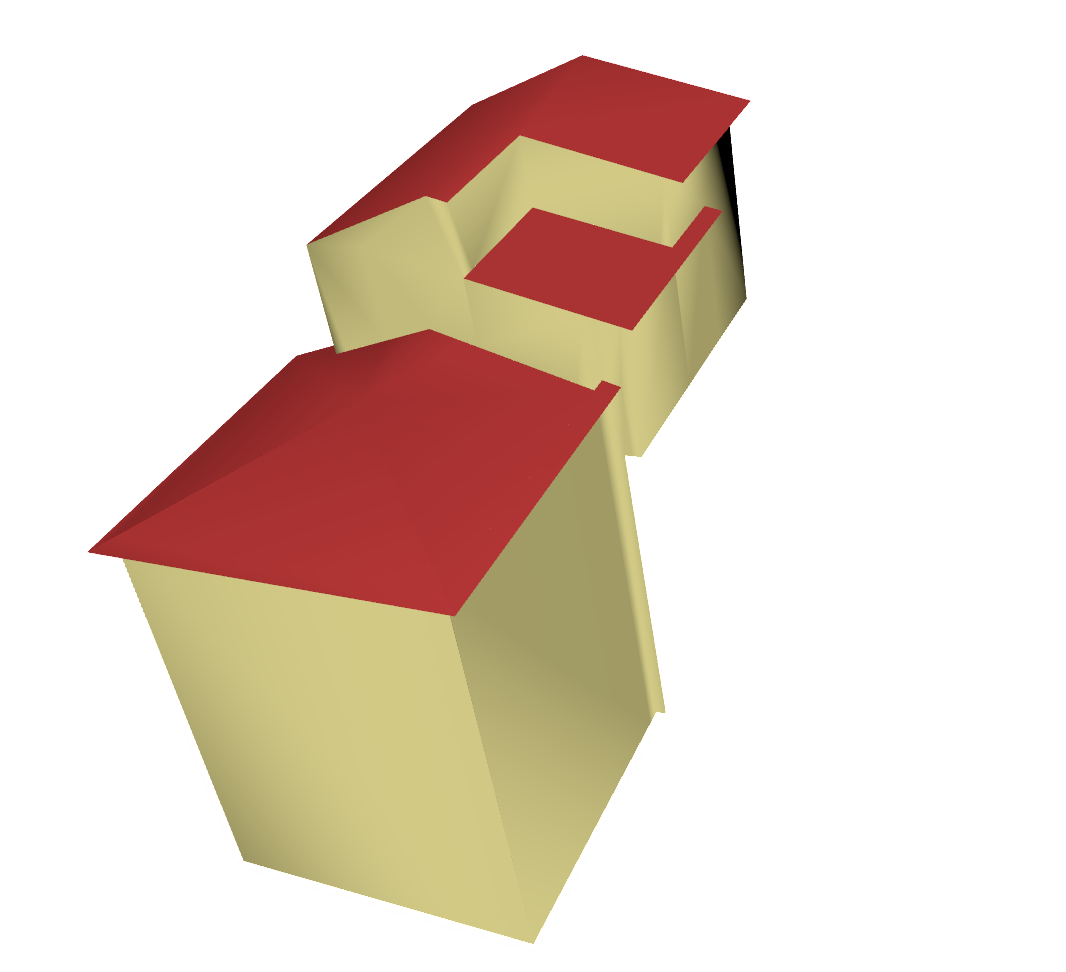
\includegraphics[width=0.5\textwidth]{chapter2/images/swisstopoBuildingModel}
\caption{A 3D--Model of a building provided by the Swiss Geospatial Portal and used in 3D--Tiles}
\label{fig:swisstopoBuildingModel}
\end{figure}
For this reason, during the last period of the development of \applicationName, models of the city of Lugano have been bought. The use of these models may be done as one of the future developments of this application. This will be discussed at the end of this report.
%%%%%%%%%%%%%%%%%%%%%%%%%
%%%%%%%%%%%%%%%%%%%%%%%%%
\section{\applicationName} \label{projectDesign}
%%%%%%%%%%%%%%%%%%%%%%%%%
\subsection{Environment and Frameworks}
The environments selected to develop \applicationName\ are the following:
\begin{itemize}
	\item {\bf The Server--side} was written using the {\bf Java} Programming Language. The {\bf Spring Framework} was used, in particular using its most famous convention--over--configuration, called {\bf Spring Boot}. The database used to store the information about the city is {\bf MySQL}.
	\item {\bf The Client--side} was written using the {\bf Javascript} scripting language. The {\bf jQuery} library was used and, of course, {\bf HTML5} and {\bf CSS3}. As mentioned above, the 3D visualization of the city was achieved using the {\bf Cesium Framework}
\end{itemize}

\subsection{The Overall Structure}
Figure \ref{fig:project_structure} shows how the final prototype of \applicationName\ looks like.
\begin{figure}[H]
\centering
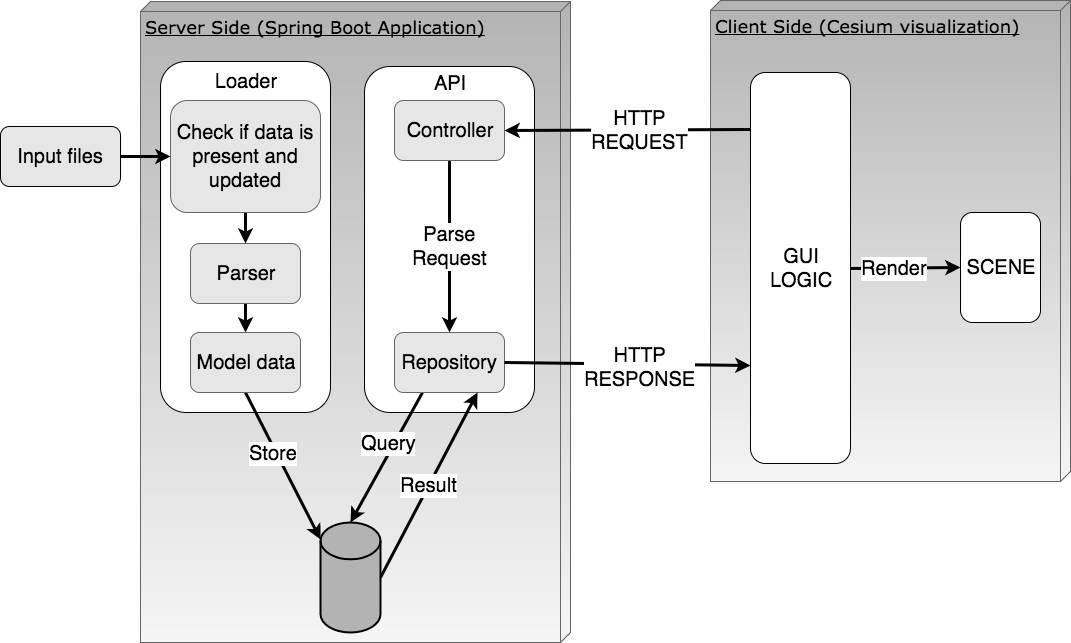
\includegraphics[width=0.8\textwidth]{chapter3/images/project_structure}
\caption{\applicationName\ architecture scheme}
\label{fig:project_structure}
\end{figure}
The upcoming sections, illustrate \applicationName\ and how it was developed. The first part proposes the \applicationName\ modelling of data. Afterwards a section about the parser and the cron--jobs created is present. Followed by a description of the API provided to the user. Finally it concludes with some discussions about how the structure and the logic behind the Web--Application was developed.
\subsection{Server Side}
\subsubsection{Available Data and Modelling}
The entire work starts from the ``xml'' file provided by the Comune of Lugano. The first choice to take was how to model the available data in the best way such that the way of retrieving information about any building was as fast and as consistent as possible.\\
The models created are the following: City, Suburb, Building, Address and Type.Figure \ref{fig:db_structure} shows, in the form of an ER diagram, the final version of how the data was modelled into the database, specifying columns and relations between tables.
\begin{figure}[H]
\centering
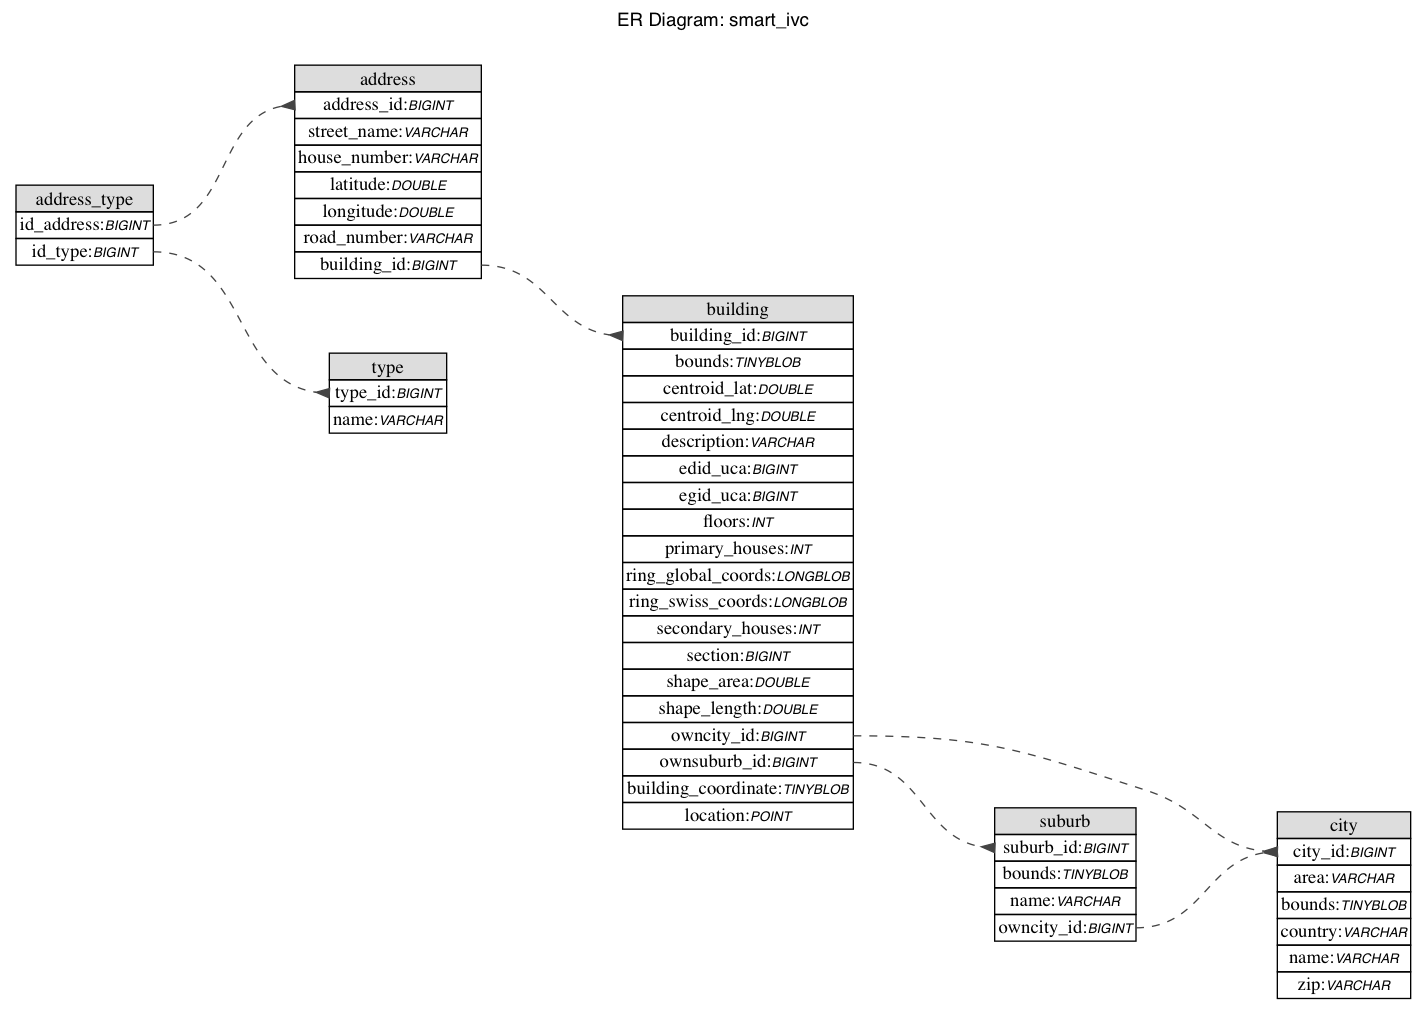
\includegraphics[width=0.8\textwidth]{chapter3/images/db_structure}
\caption{\applicationName\ database structure}
\label{fig:db_structure}
\end{figure}
\subsubsection{Parser}
The data type taken as input is of xml type. It is used in the process to load buildings data.\\
At the beginning of the file an header which describes the content is defined. It regulates fields and types as well as values range, tolerances in the coordinates system and other set ups parameters. After the header, a long record of elements which represent buildings follows (exactly 18904). Structure and constraints, of record elements are defined in the header. The record presents several data, out of this data  \applicationName\ finds use on almost all of them. Here there will be described the tags that can be found in the xml file and that were found useful for \applicationName\:
\begin{itemize}
	\item {\bf SHAPE:} it stores both the perimeter of the building and the max bounds that it occupies
	\item {\bf Descrizione:} it represents the type of the building. Between them only the ones of type ``Edificio'' (i.e., building in Italian), are stored
	\item {\bf Sezione:} it is a numeric value that represent the suburb in which the building is located
	\item {\bf NUM$\_$CIVICO$\_$ID:} it is a 8--character--long numeric value that contains: the number id representing the street name in the first four characters and the civic number in the remaining four.
	\item {\bf EGID$\_$UCA:} it uniquely identifies buildings on the entire Swiss ground on the basis of the ``Registro Federale degli Edifici e delle abitazioni'' (REA) from the ``Ufficio federale di statistica''.
	\item {\bf PIANI:} the number of floors per building
	\item {\bf SHAPE$\_$AREA:} the area of the plane described by the building
	\item {\bf SHAPE$\_$LENGTH:} the length of the perimeter of the building
\end{itemize}
The data is assimilated in \applicationName\ through the loader. A parser has been created in order to read and parse a file structured in the way described above. The parser creates a building model and an address model for every record in the xml file and sets their fields using the information stored in the xml tags. Once the data is created, the models gets stored into a database.\\

Coordinates of buildings are stored in a data type called CH1903. It represents the Swiss projection coordinates system. It uses an Oblique Mercator on a 1841 Bessel ellipsoid. An Oblique Mercator is an oblique conformal cylinder projection. Together with the 1841 Bessel ellipsoid, a reference ellipsoid of geodesy with base at the old observatory in Bern, gives meaning to the projected coordinates. The transformation computations of the data from CH1903 to WGS84 is provided from the Swiss confederation. The precision with this transformation is of respectively 1 meter and 0.1". In order to derive the transformationa specific formulae has to be applied. The way these coordinates are converted can be found on the website of the Federal Office of Topography Swisstopo under the section NAVREF. 
\subsubsection{Commands}
On the application start, the application checks if the data is already present in the database, if not it executes a command that reads the xml file and parses it using the parser described above and stores the models in the database.\\  
At this point, the data is not ready yet, since it does not contain all the important information required from \applicationName\ to work.\\
That is why some commands where create for different purposes. Again, on application start, it is checked if the data is updated properly, if not the following commands are executed:
\begin{itemize}
	\item The {\bf CityLoaderCommand} contains two commands to be executed: the first one, as explained above, parses the xml and stores the models in the database. The second one, adds some additional information about the buildings (i.e., number of apartments--per--building that are primary and secondary houses). This additional information was received by the Comune of Lugano in a second time in the format of a txt file. Therefore, the matching between buildings listed in the two files was done using the EGID value. 
	\item The {\bf ConverterCommand} is used to convert the coordinate system used for the perimeters of the buildings from CH1903 to WGS84. The conversion is done using the service provided by the Web APIs of the Federal Office of Topography Swisstopo  where, given a pair of coordinates in the CH1903 system, their respective conversion in WGS84 is returned.
	\item The {\bf CityInformationCommand} is used to add additional information to each building though three different services. The first one adds information about the membership suburb using an APIs service provided by Swisstopo that uses the EGID in order to get such an information. Another service provided by Swisstopo API's is used to get information about the address name and the civic number of the building, still using the EGID value. The last command uses the API service provided by OpenStreetMaps in order to get information about addresses, civic numbers (for the building that have not an EGID value stored) and type of the building (e.g., Hospital, School, University etc \dots).  
\end{itemize}
Once these commands are executed, the data is ready to be used and retrieved in order to be shown on the web application.
\subsubsection{Controllers and Queries}
Once the data was retrieved from the xml, modelled, improved with additional details and correctly stored in the database, the only part missing on the server side was the creation of the APIs and the correlated work of querying the database to get the correct information.\\
\begin{center}
	\cfbox{red}{SECTION WORK IN PROGRESS (how much be detailed on controllers specifications?)}
\end{center}

\subsection{Client Side}
\subsubsection{The first Attempt: Babylon.js}
Immediately after having gathered the essential data useful to draw the buildings of the city of Lugano, a first attempt of visualizing them was made using BabylonJS. It is a JavaScript framework for building 3D environments with HTML5 and WebGL. It allows the creation of a scene with customized lights, cameras, materials, meshes, animations, audio and actions. It also supports scene picking (i.e., an element on the scene is clickable and it is possible to interact with it).\\

In order to test the capabilities of BabylonJS, a small portion of Lugano (i.e., the part around the lake) was selected and rendered. The result can be seen in the following image:
\begin{figure}[H]
\centering
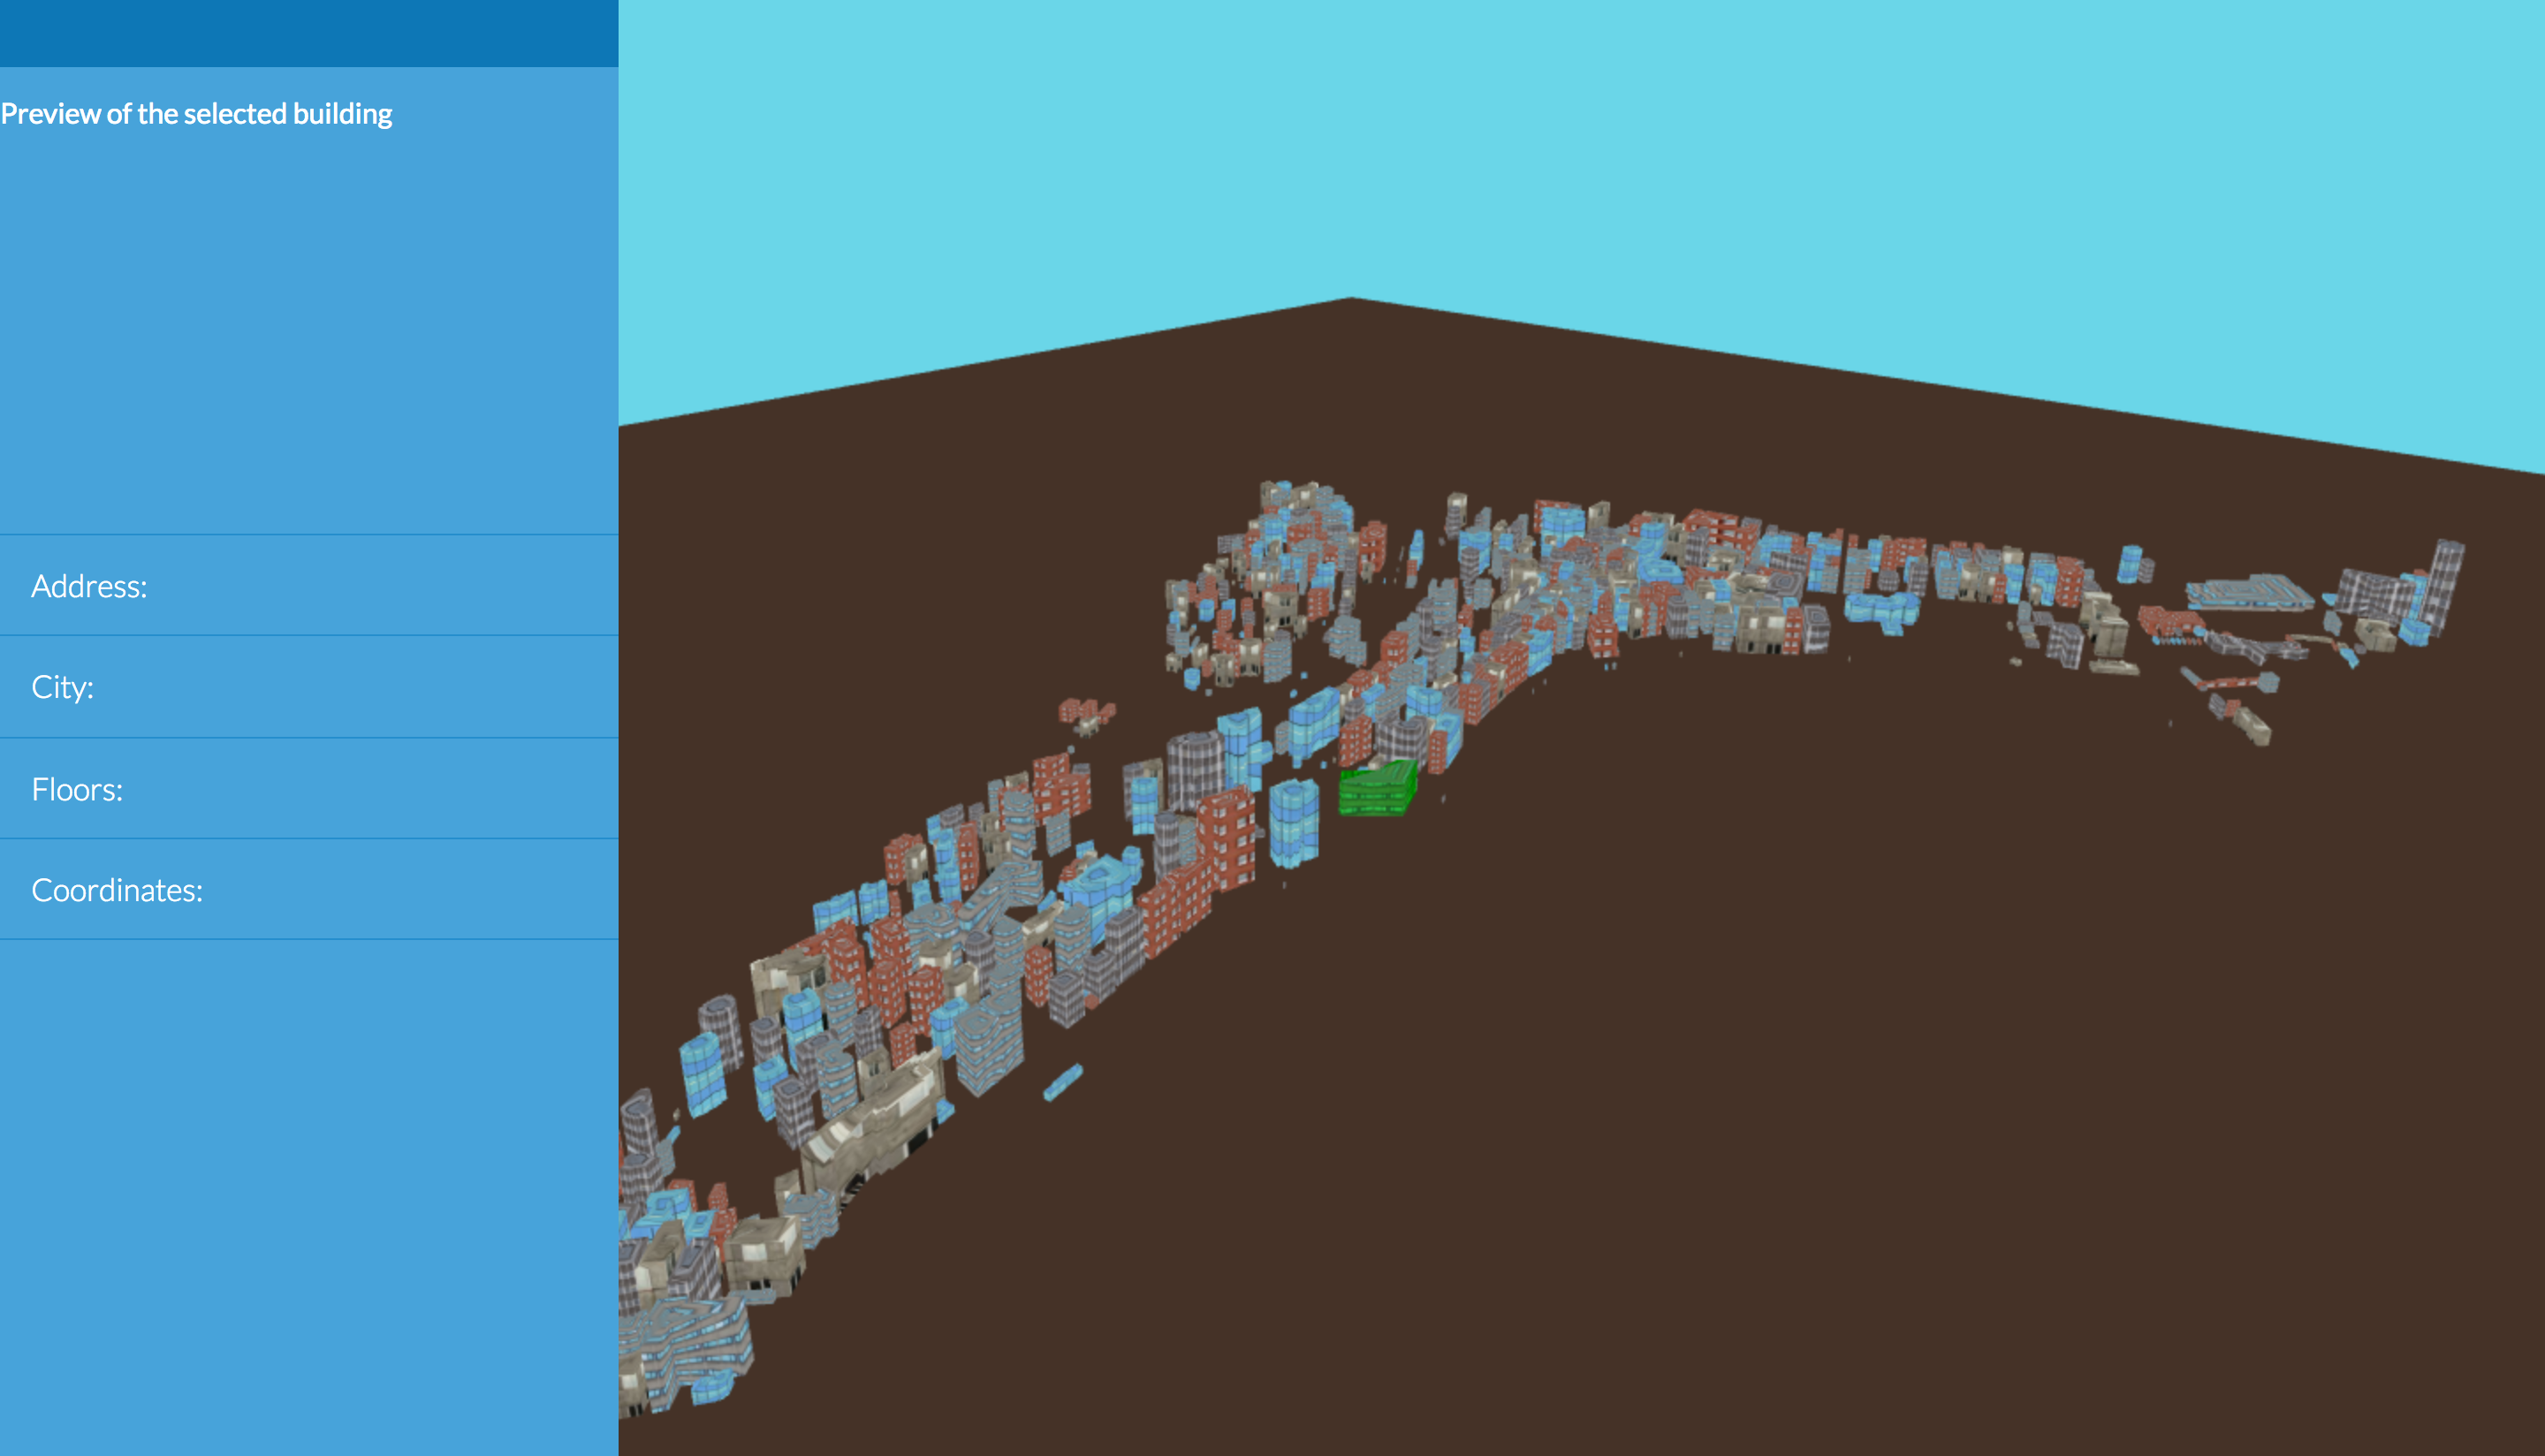
\includegraphics[width=0.8\textwidth]{chapter3/images/babylonJS}
\caption{The first attempt of city visualization using BabilonJS}
\label{fig:babilonJS}
\end{figure}
As long as the buildings showed in the scene where under the two--thousand, the browser was very fast in rendering during the loading of the page and the movement of the camera was smooth.\\
The main problems that make the idea to use BabylonJS discarded, were has been basically two:
\begin{itemize}
	\item The buildings to be rendered were far above the mentioned threshold, the rendering would take more than 30 seconds.
	\item BabylonJS provides no basis to start from: the initial scene is completely empty and, as it is possible to see in the image above, buildings lay on a plane. That represented a serious problem since the visualization of the city was planned to be shown in a way that would be as realistic as possible.
\end{itemize}
A solution to the last problem would have been using the Google Elevation API. This service, given a pair of coordinates (i.e., latitude and longitude), returns the exact altitude of that point.\\

Unfortunately, the API system of Google provides just 2,500 free requests per day. In the case of Lugano, that extends its territory for more that $25km^2$, considering one request for meter it would have been taken more than 10 days to get the entire terrain structure (for the entire city of Rome, that spans almost $46km^2$, the days taken would have been more than 20).\\

Nonetheless, this would have made the rendering slower since, in addition to the visualization of the buildings, also a rendering of the terrain (i.e., lakes, mountains and rivers) would have taken place.\\
Therefore, this lack of both Google--API--requests and good performances, lead the idea to use BabylonJS to be discarded.
\subsubsection{The final version: Cesium.js}
As stated above, the Cesium Framework was finally used to build the client--side of the application.\\
Cesium, on the contrary, provides a ready--to--use virtual globe
\begin{center}
	\cfbox{red}{SECTION WORK IN PROGRESS}
\end{center}

\subsubsection{Provided Interface}
\applicationName\ aims to create interactive 3D cities representations accessible by everyone. In order to have interactions that may suggest interest in users, it is required to have an user--friendly system which allows interactions with the entities in the city. In order to achieve this feature in the most flexible way, a tab based interface is at disposal of the user. The proposed interface is composed as follows:
\begin{itemize}
	\item An {\bf Info--Box} is shown whenever a building is selected. All the available information about it are displayed such as: street name, civic number, membership suburb, number of floors, purpose of the building and Percentace of Primary and Secondary Houses.
	\item A {\bf sidebar} is at user's disposal and it is divided into the following subsections:
	\begin{itemize}
		\item The {\bf Visualize} Tab let the user: {\bf add elements} to the city like the geolocalization and the position of the cameras distributed around the city, {\bf color} the city by height or by suburb and decide to {\bf show some suburbs} rather than others.
		\item The {\bf Query City} Tab is the core of the interaction between the user and the city visualization. It is possible to create a completely personalized query, selecting which field to search and which value should be searched. This part will be better explained later in this report.
		\item The {\bf Query History} Tab contains the list of all the queries executed during the session, showing the number of results for every different query.
		\item The {\bf Credits} Tab just contains information about who worked on this project and what technologies were used for the 3D--visualization.
	\end{itemize}
\end{itemize}
\subsubsection{Query Builder}
\subsection{Potential and Limit}
%%%%%%%%%%%%%%%%%%%%%%%%%
%%%%%%%%%%%%%%%%%%%%%%%%%
\section{Use Cases} \label{useCases}
%%%%%%%%%%%%%%%%%%%%%%%%%
In this chapter some of the possible actions that can be performed into \applicationName\ are presented. The aim of this chapter is to provide a practical introduction to \applicationName, through different use cases.
\subsection{Access information}
The first use case presented introduces the available option to access building models data.\\
An InfoBox is shown, whenever a building is selected through a click of the mouse or a tap on the screen of a smartphone. Figure \ref{subfig:infoBox} and Figure \ref{subfig:infoBox_city} shows how these information are given to the user.\\
\begin{figure} [h]
\centering
	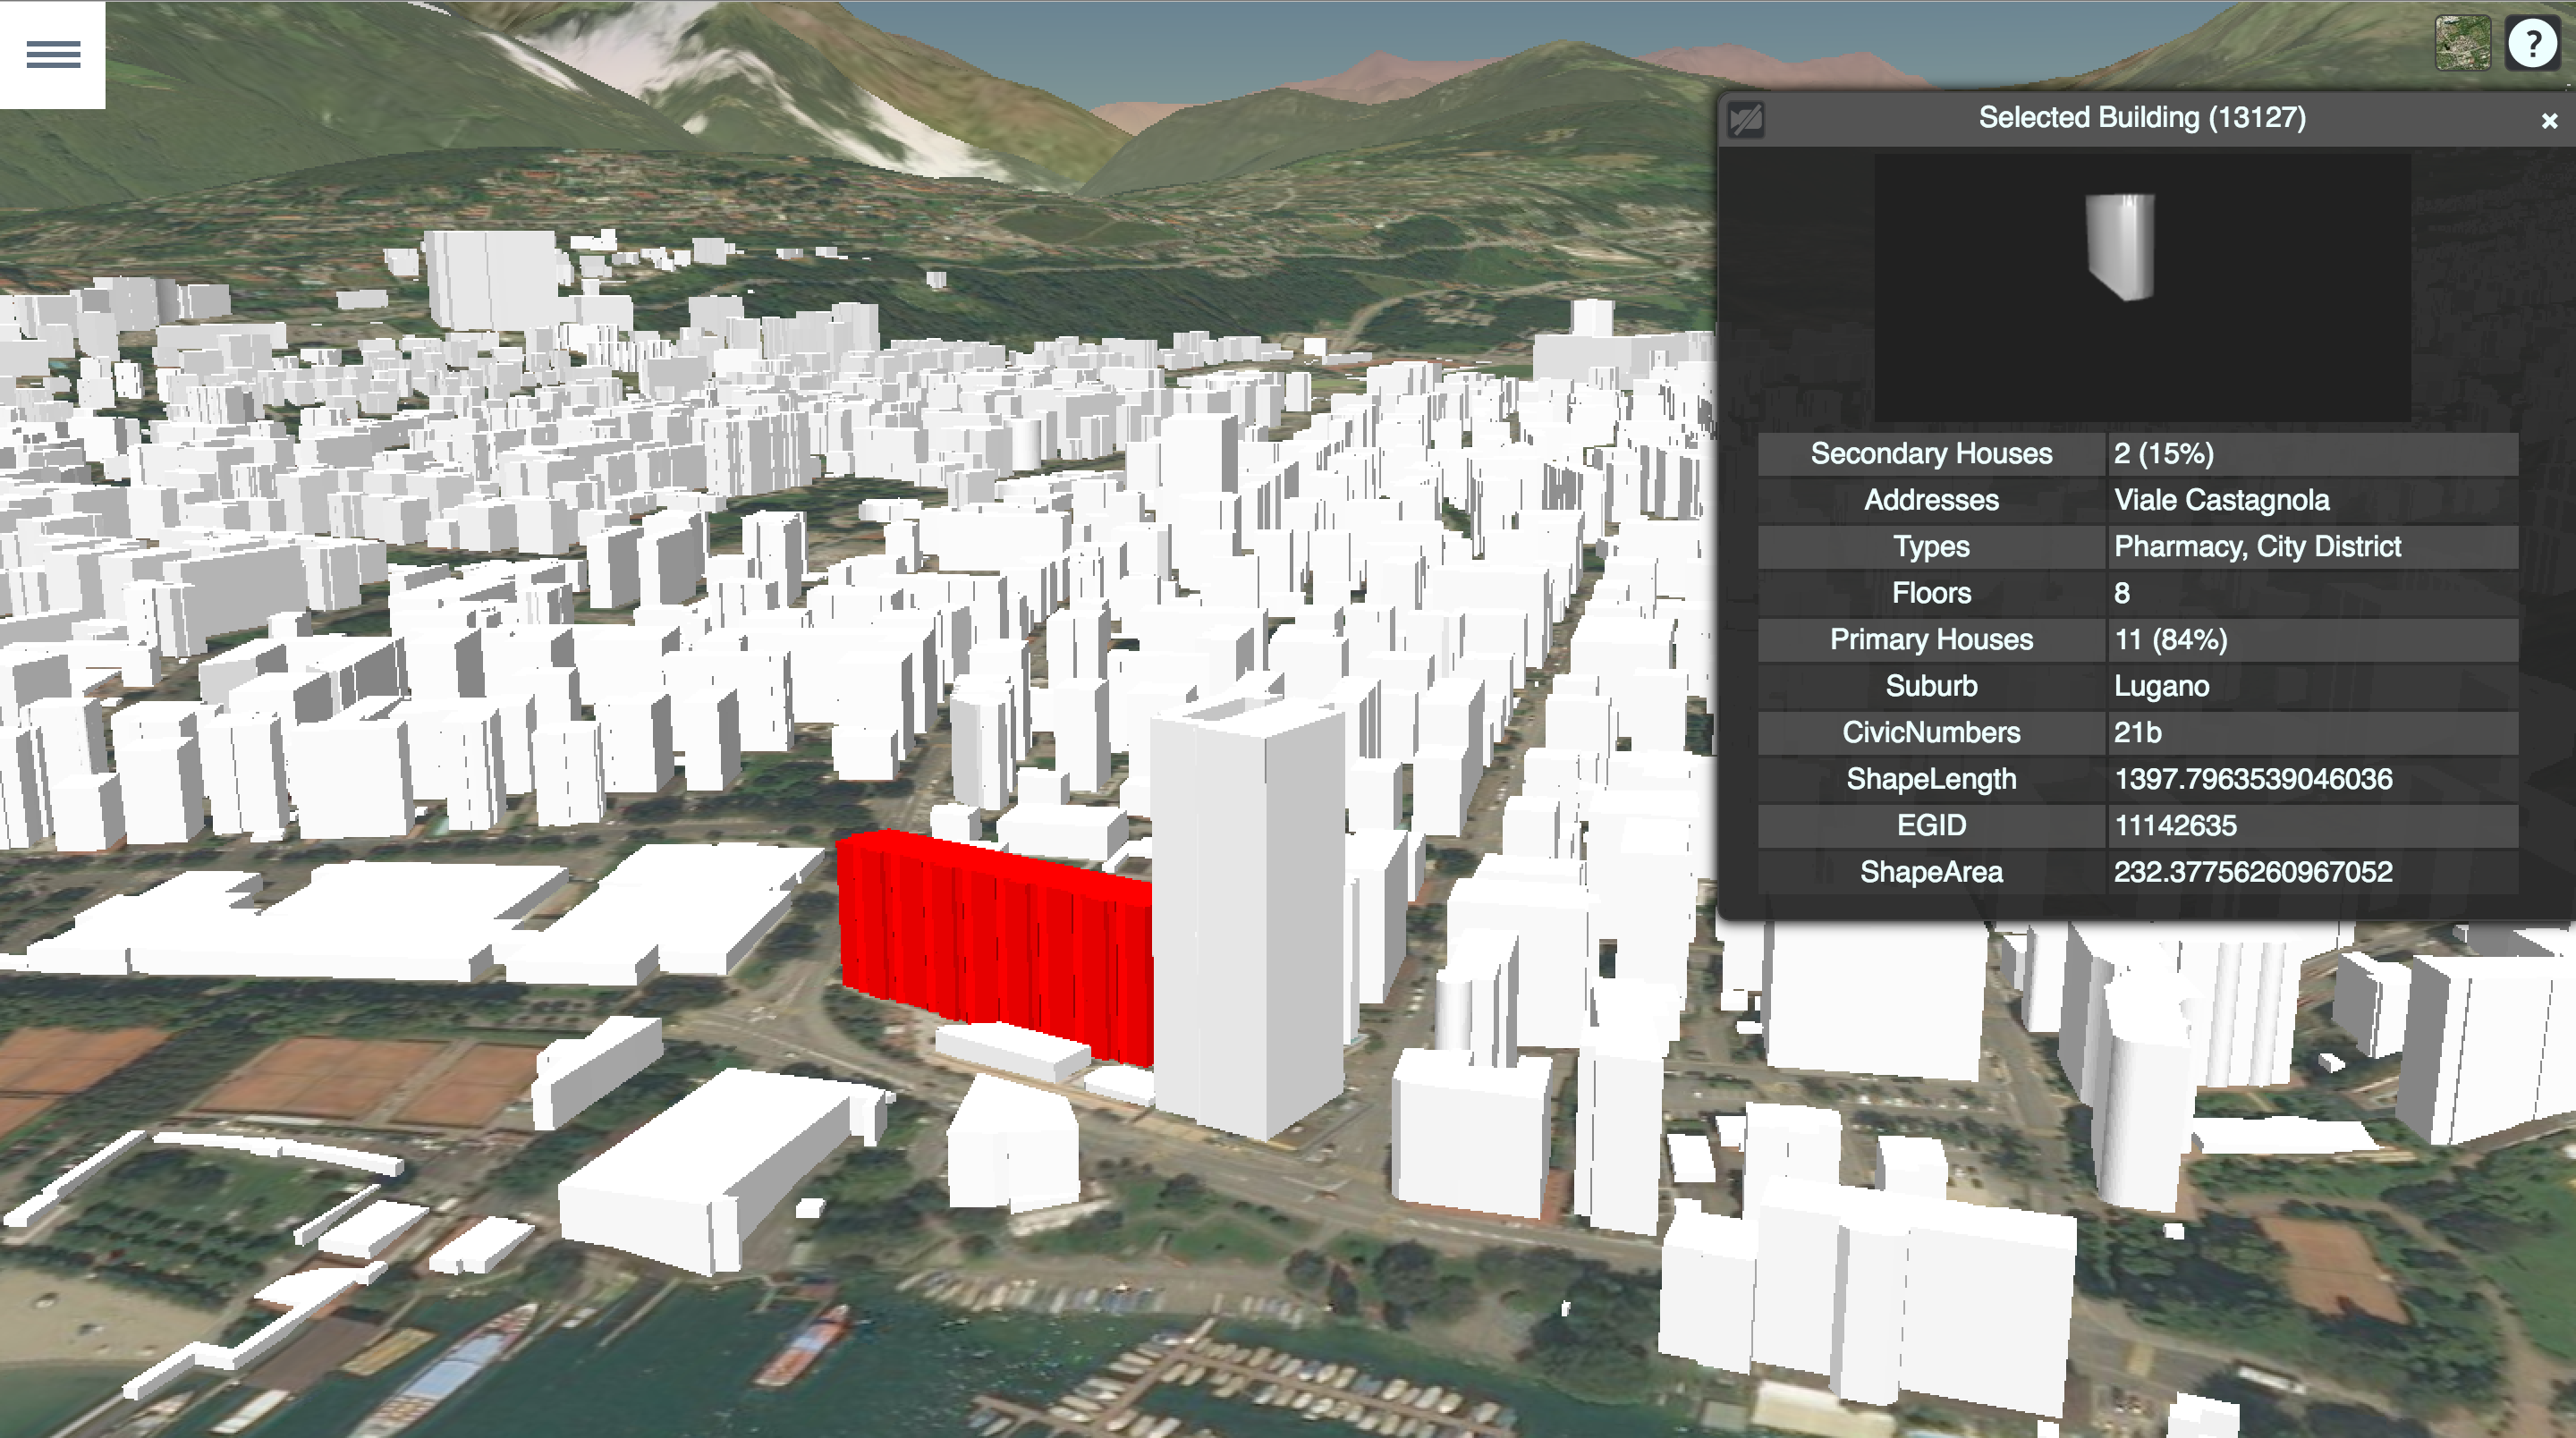
\includegraphics[width=0.8\textwidth]{chapter4/images/infoBox_city}
	\caption{Selecting a building will make the InfoBox appear automatically}
	\label{subfig:infoBox_city}
	\end{figure}
\begin{figure} [h]
	\centering
	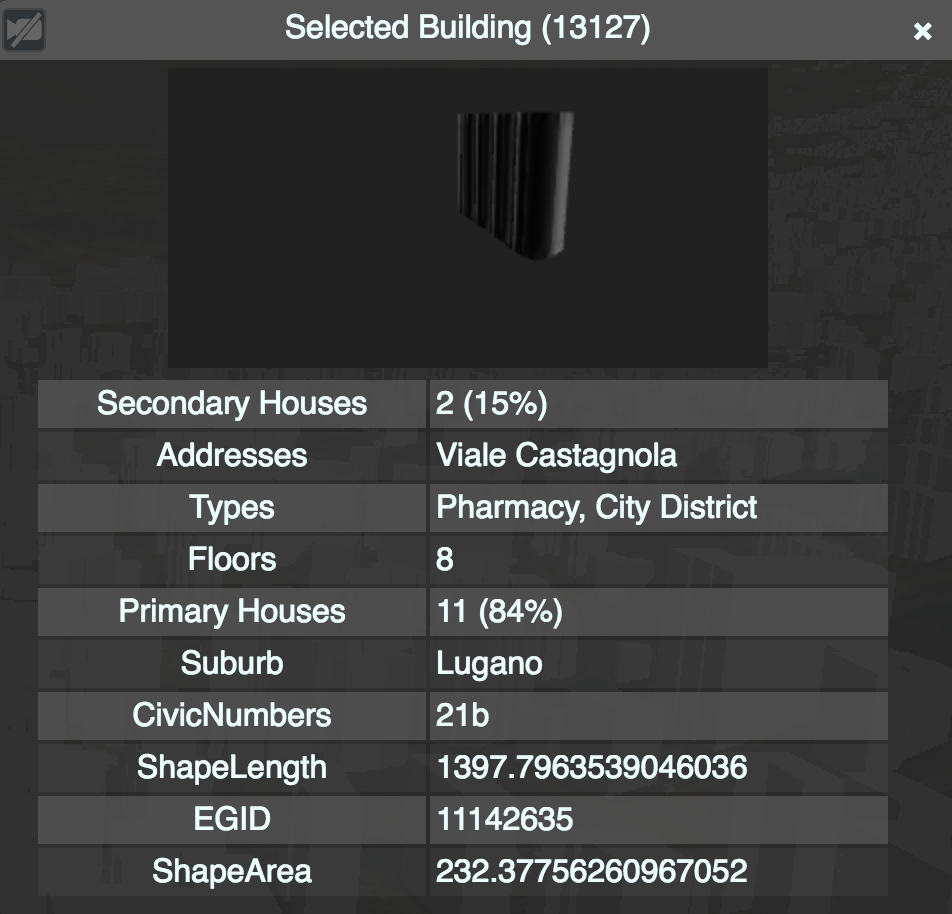
\includegraphics[width=0.5\textwidth]{chapter4/images/infoBox}
	\caption{A detailed look at the InfoBox}
	\label{subfig:infoBox}
\end{figure}
The first field displayed is a 3D representation of the model of the building clicked without its surrounding environment. It is possible to interact with this canvas in order to rotate and zoom the building model freely.\\
After, a list of useful information about the building follows: the length of this list changes from building to building depending on the availability of the information.\\
The building clicked in the example of figure \ref{fig:infoBox} presents all the possible available information that an user can get about a building.\\
The fields of the displayed data are denoted as follows: 
\begin{itemize}
\item {\bf Types} provides the list of groups in which the building is present. Groups are defined by the OpenStreetMap APIs and are used to represent the usage of the buildings which, conceptually, have characteristics in common. Examples of types are: Post Office, Pharmacy, Hospital, University etc \dots.
\item {\bf Floors} is the number of floors that the building possesses
\item {\bf Shape Length \& Shape Area} represent the size of buildings available for consultancy, they are measured in length and area both expressed in meters.
\item {\bf Street Name \& Civic Numbers} are the data concerning the addresses of the street where the building is located. There could be more than one street name and civic numbers in case the building has many of them (e.g., different entrances in the same building that are on different streets). Addresses data are taken from Swisstopo APIs and, if not available from this service, OpenStreetMap APIs are used.
\item {\bf EGID} the unique identifier of the building given by the Swiss REA 
\item {\bf Suburb} represents the suburb in which the building is located
\item {\bf Primary \& Secondary houses} represents both the number of primary and secondary houses in the selected building and the percentage that each value represents over the total number of houses in that building
\end{itemize}

\subsection{Visualize the City}
The first tab available to the user when the side--bar is opened, is the Visualize Tab. It is divided into three main subsections: ``Show on the map'', ``Color city'' and ``Show Suburbs''.\\

The first subsection contains two checkboxes: the first one, let the user show the geolocalization, i.e., the position of the device from which the user is using \applicationName. The second checkbox, if checked, shows the position of webcams located around Lugano; this webcams continuously stream videos of the city. In Figure \ref{fig:mapPins} it is possible to see the result on the map, when both checkboxes are checked.
\begin{figure} [H]
\centering
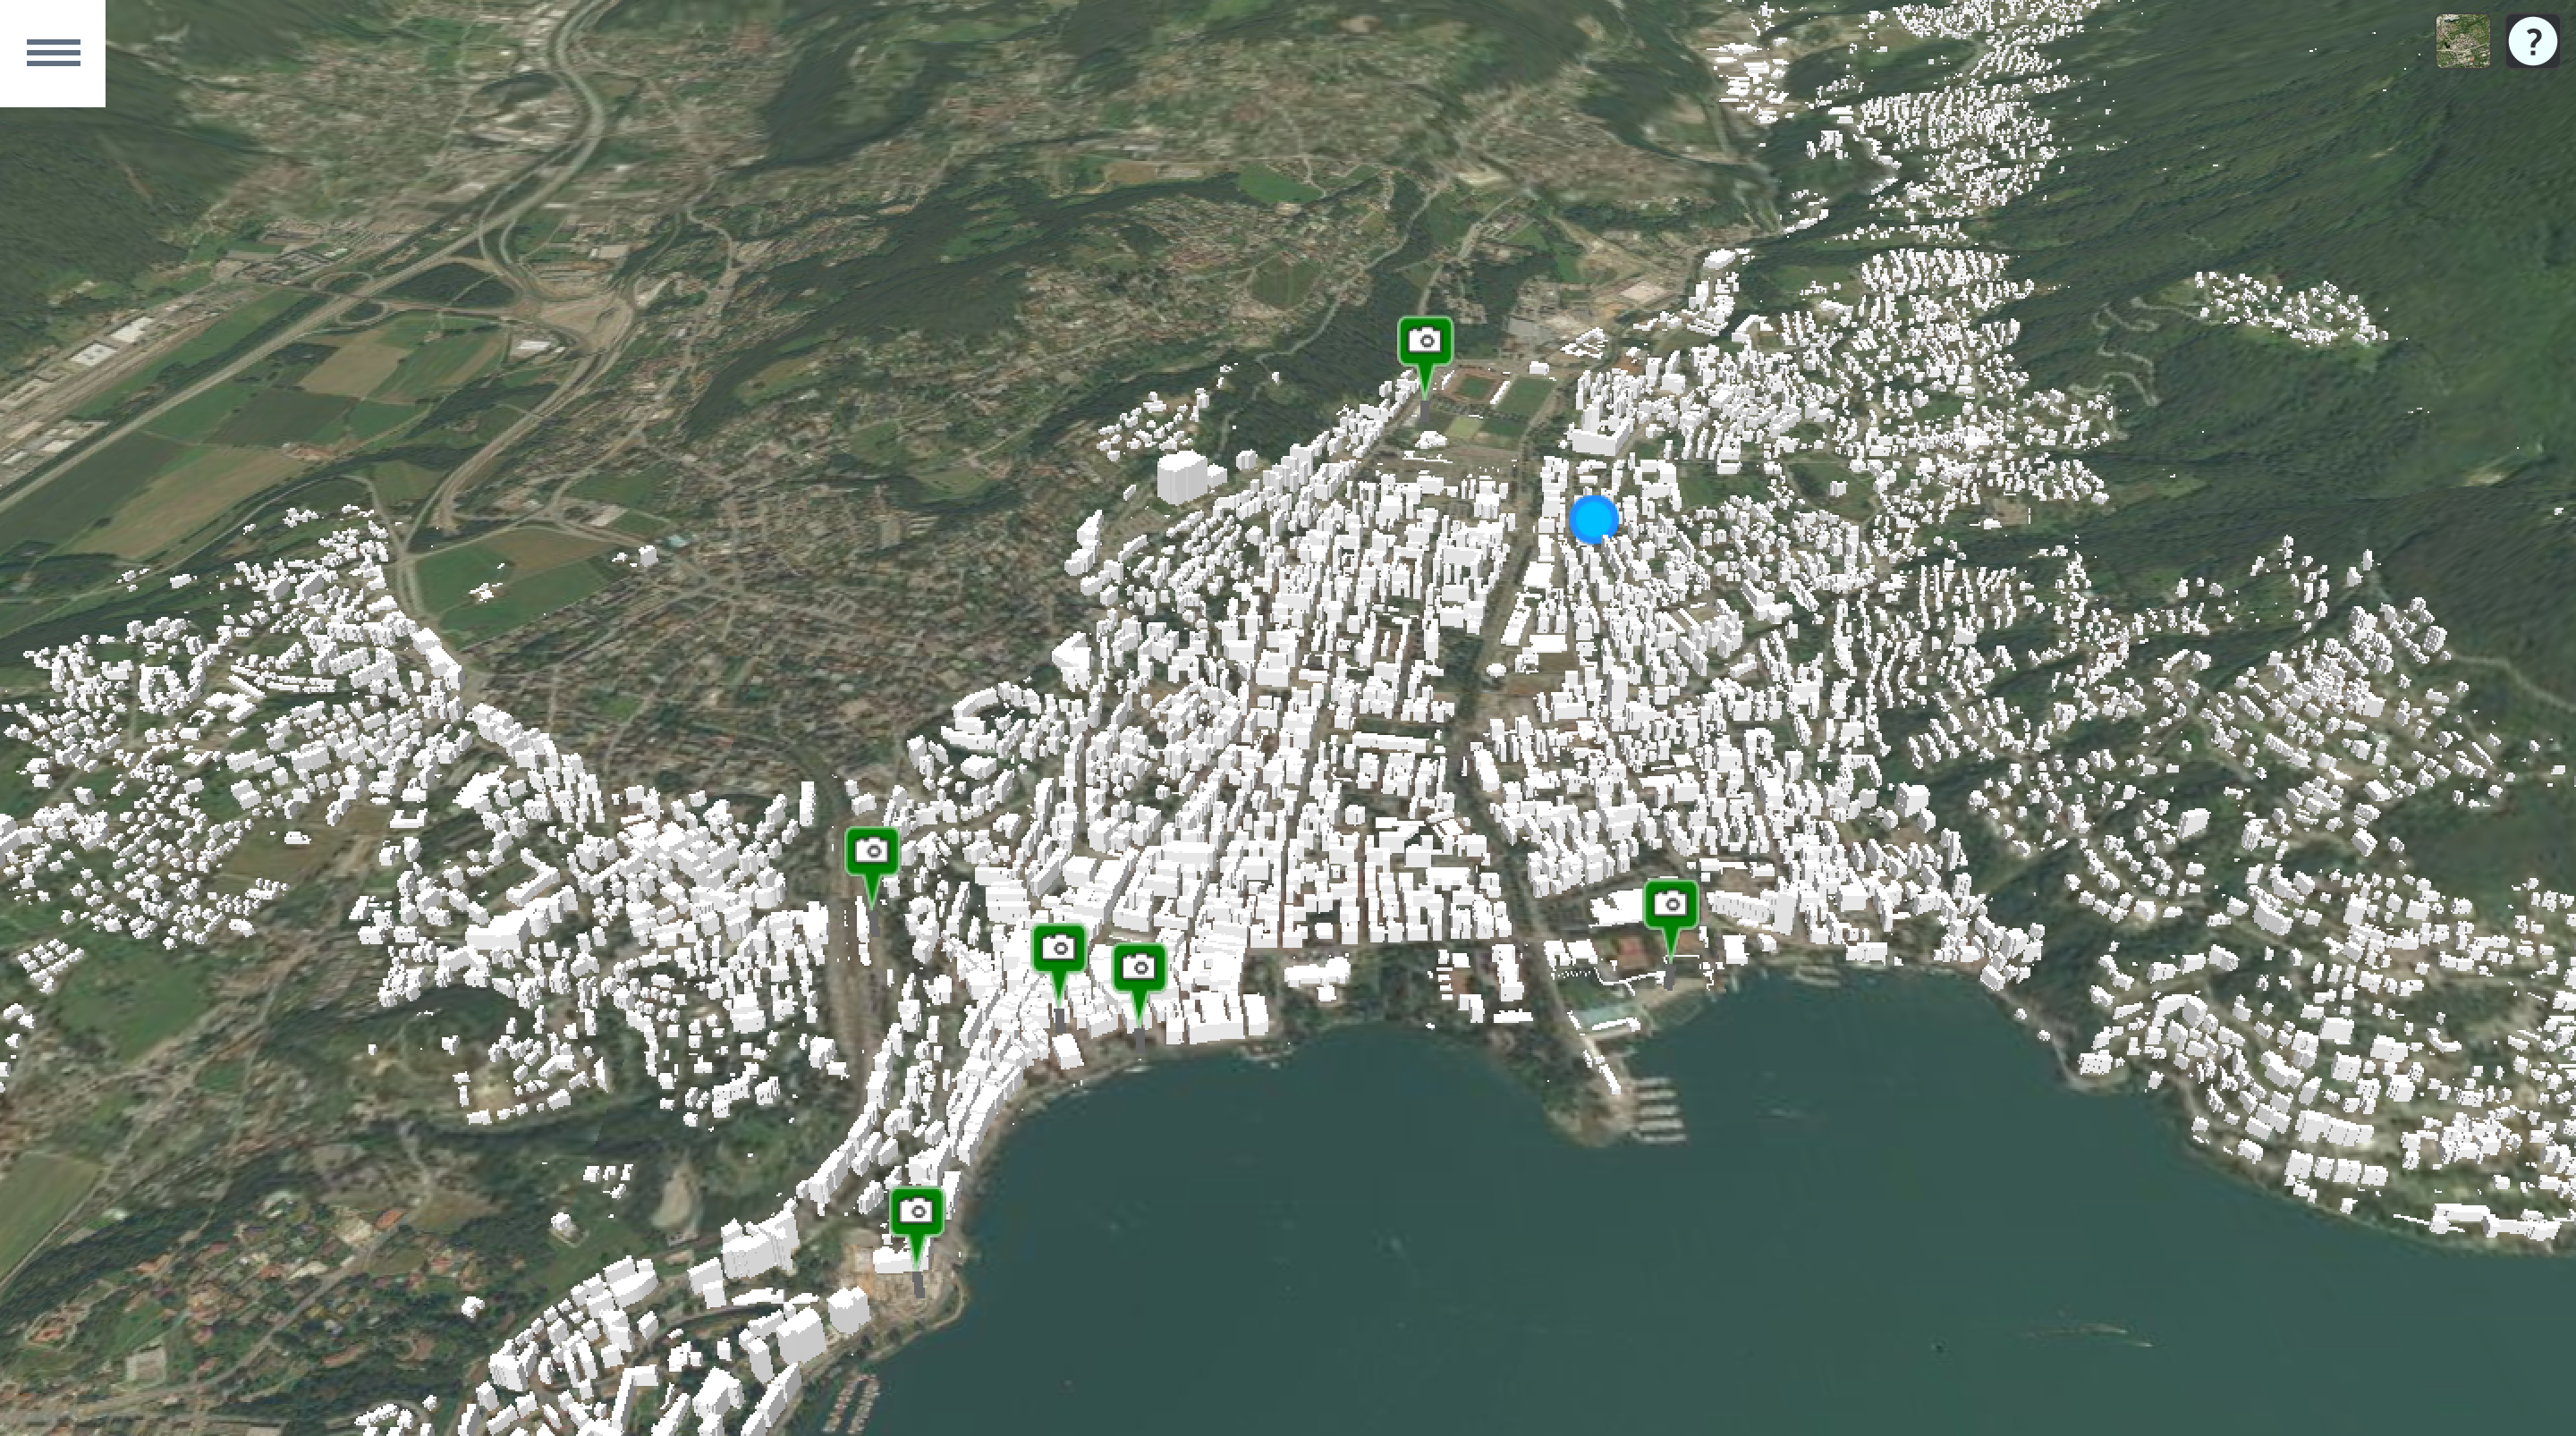
\includegraphics[width=.8\textwidth]{chapter4/images/mapPins}
\caption{When both checkboxes are checked, geolocalization and webCams positions are shown on the map}
\label{fig:mapPins}
\end{figure}
Since the 3D visualization had still to allow the user to exactly locate the position of these pins, whenever the visualization is more zoomed it it, a ``stick'' is created starting from the ground and ending at the bottom of the pin, as it is shown in Figure \ref{fig:3dPins}.\\

\begin{figure} [H]
\centering
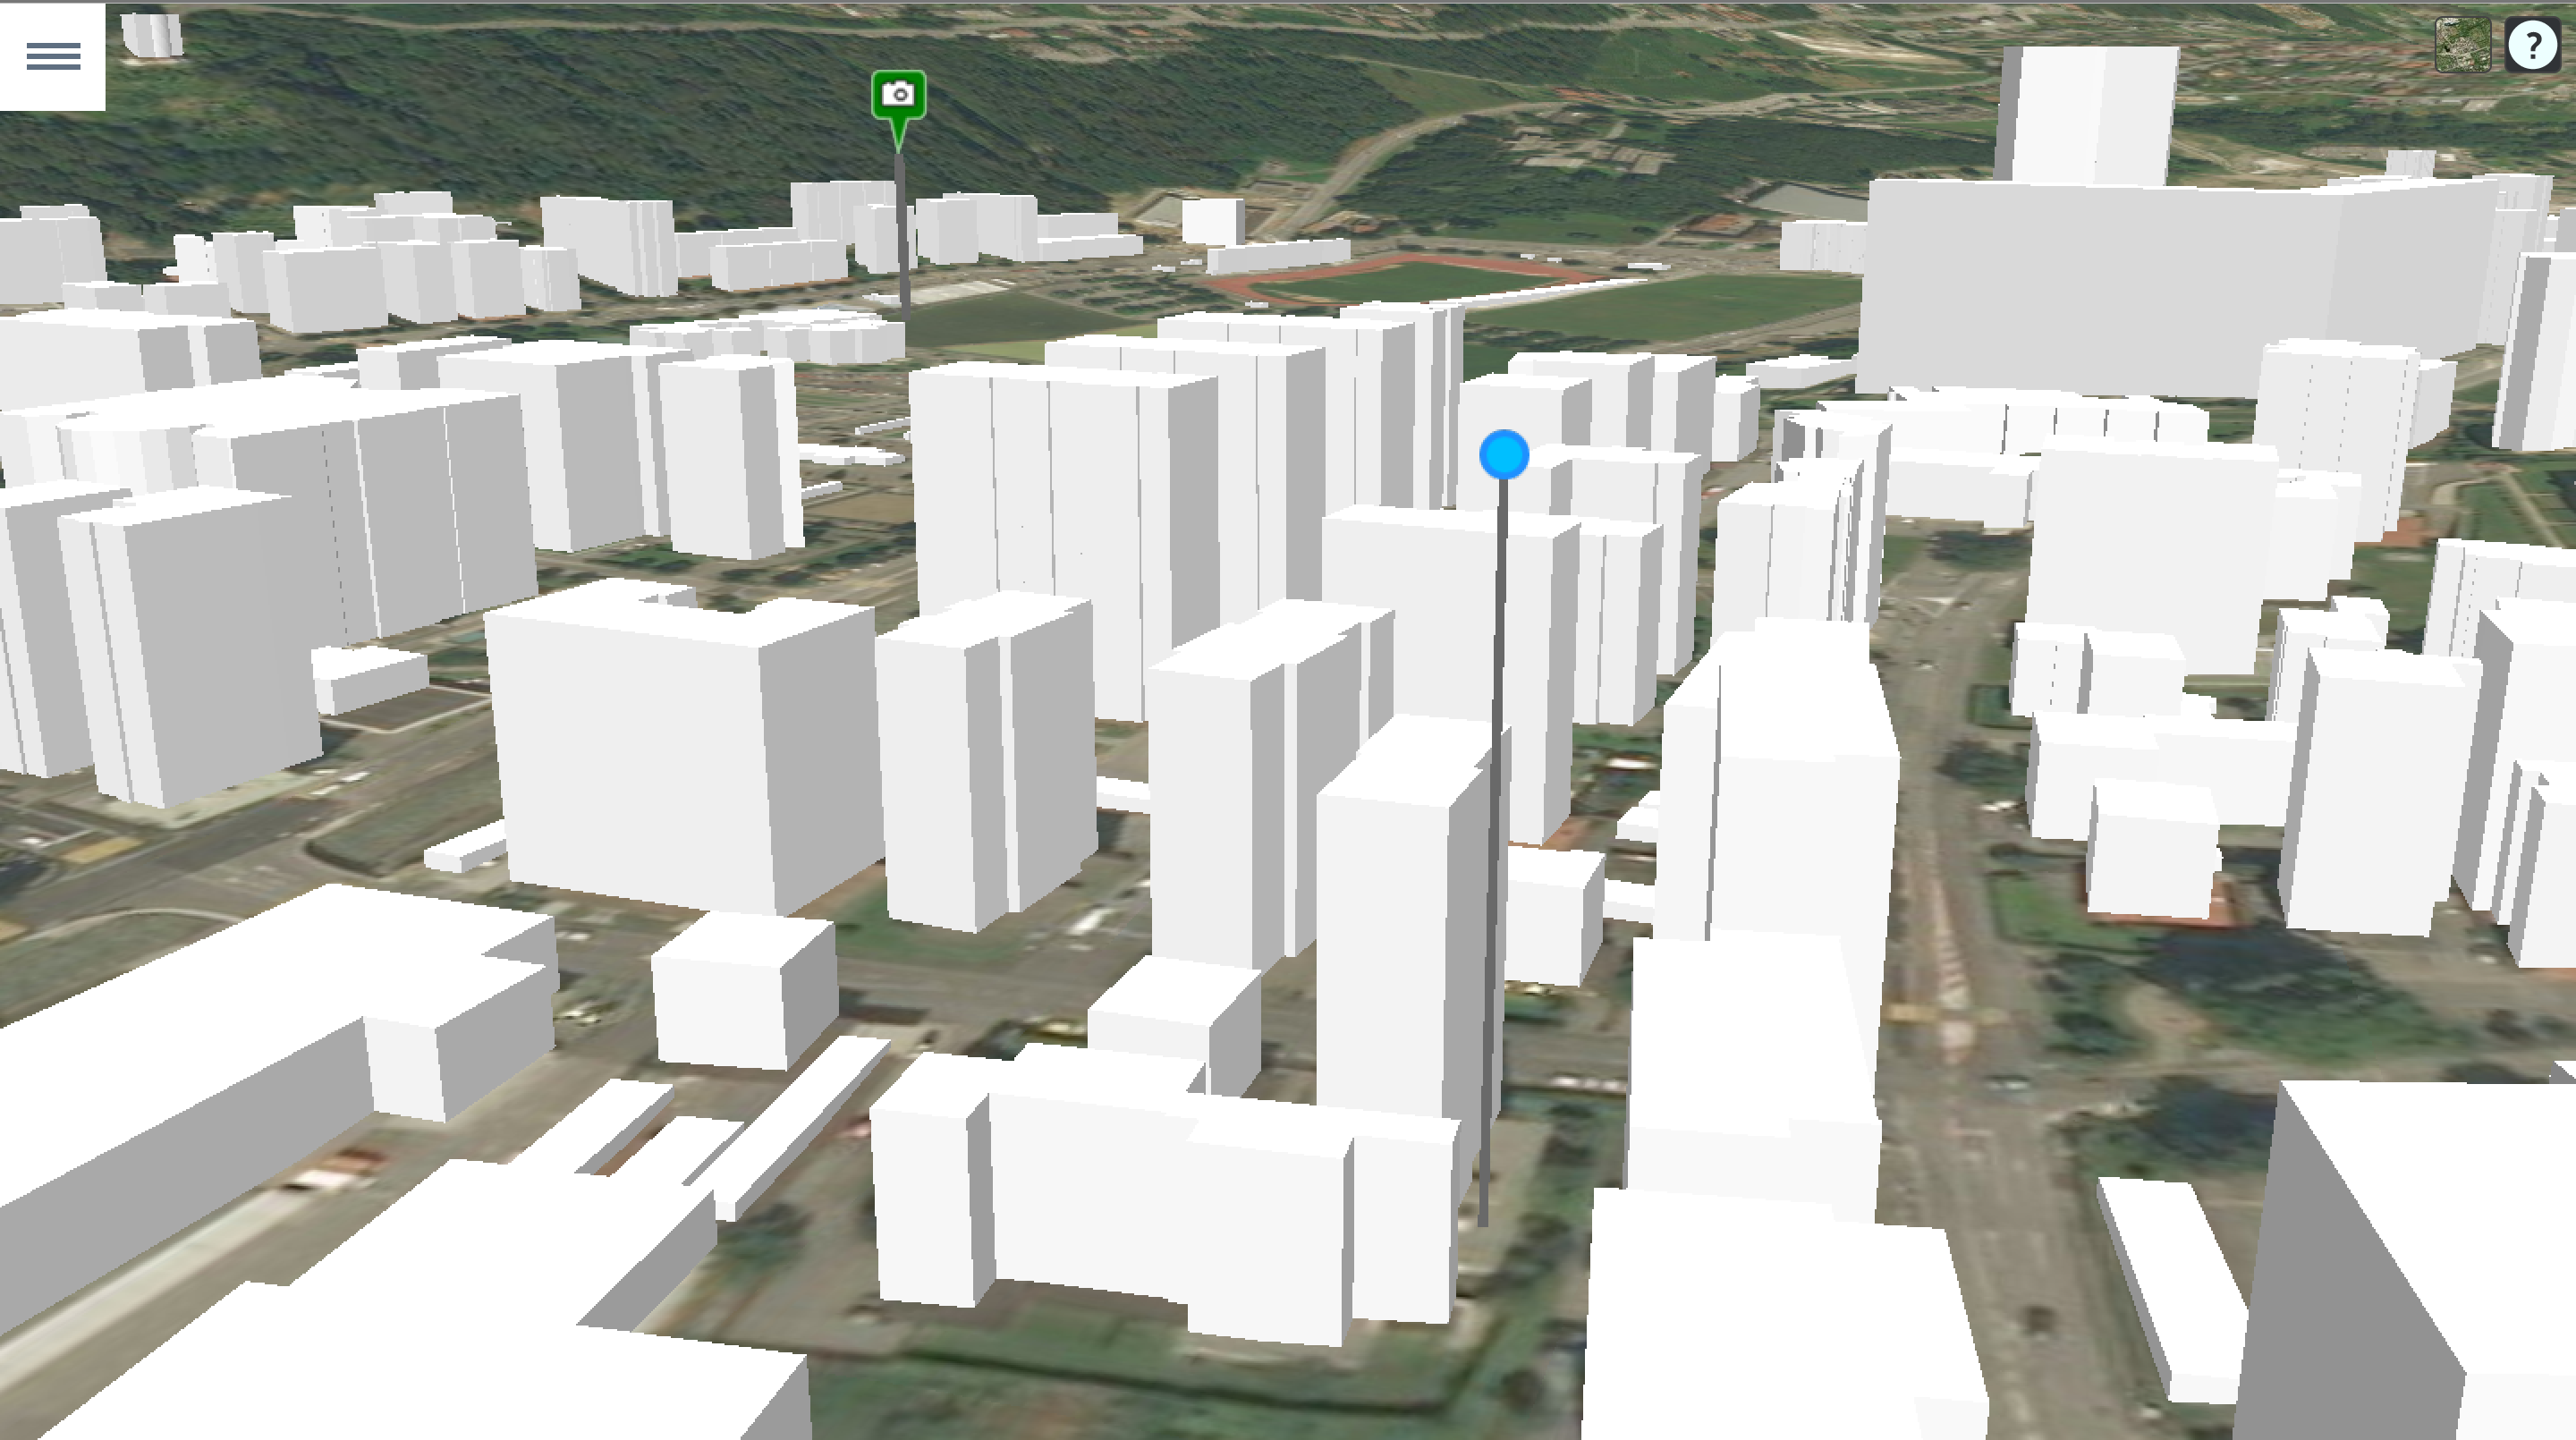
\includegraphics[width=.8\textwidth]{chapter4/images/3dPins}
\caption{The ``Stick'' that connects the ground to the pins}
\label{fig:3dPins}
\end{figure}
In the second subsection three radio buttons can be found: the first one is used to reset the color of the entire city to the default color. The second colours the buildings in the city based on their height (Figure\ref{fig:application_byHeight}). The third one is used to colour the entire city based on its suburbs and so every suburb has a different color(Figure \ref{fig:application_showSuburb} ).\\

\begin{figure} [H]
\centering
\includegraphics[width=.8\textwidth]{chapter4/images/application_bySuburb}
\caption{A Visualization of the city of Lugano where every suburb is coloured differentrly}
\label{fig:application_bySuburb}
\end{figure}
\begin{figure} [H]
\centering
\includegraphics[width=.8\textwidth]{chapter4/images/application_byHeight}
\caption{A Visualization of the city of Lugano where every building is colorued based on its height}
\label{fig:application_byHeight}
\end{figure}
The third and last subsection, contains the list of checkboxes representing all the suburbs in the city and their respective colours. By default all checkboxes are checked but uncheck them will result in hiding the desired suburb as show in Figure \ref{fig:application_showSuburb}.
\begin{figure} [H]
\centering
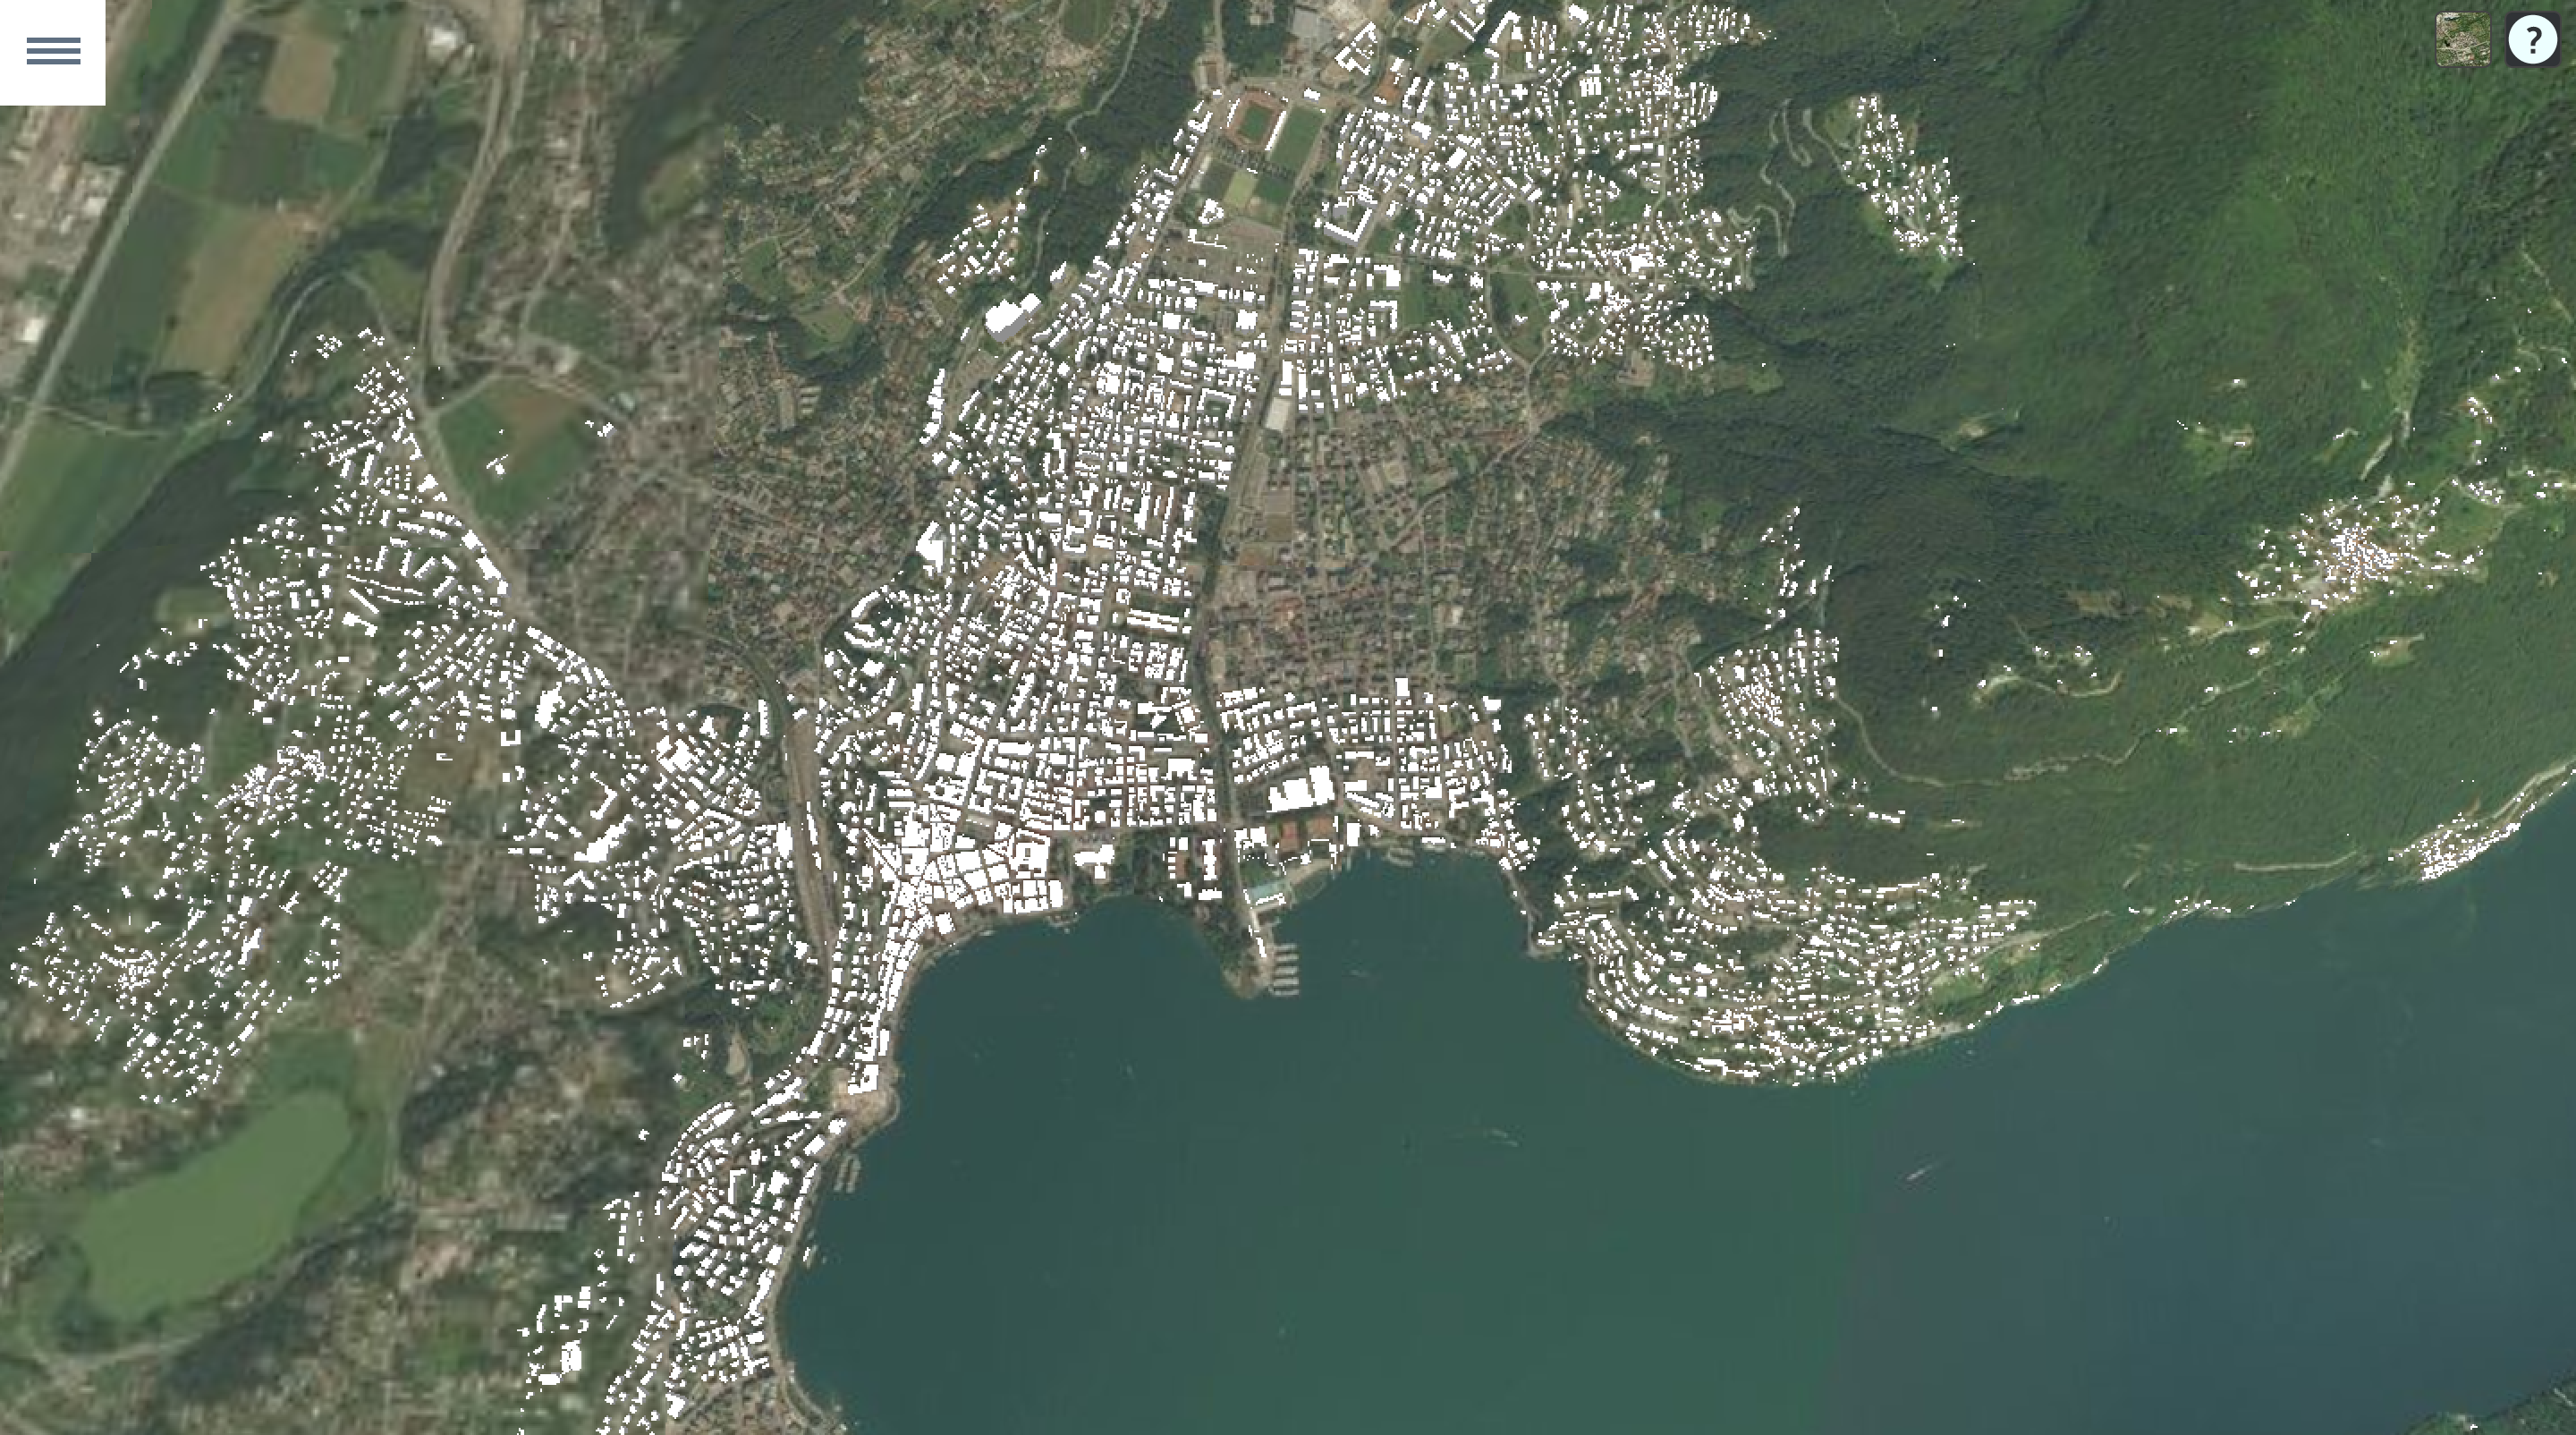
\includegraphics[width=.8\textwidth]{chapter4/images/application_showSuburb}
\caption{A Visualization of the city of Lugano where the suburb Viganello is hidden}
\label{fig:application_showSuburb}
\end{figure}

\subsection{The Query System}
\subsubsection{Building Selection}
The following use cases show what actions can be performed using the visual query system. The interactions proposed are accessible through the apposite ``Query City'' selection tab in the provided sidebar.\\
As it is possible to see on Figure \ref{fig:query_city_tab} in the previous chapter, \applicationName\ allows the user to perform from very single to more complex query on the entire city. Some examples are shown in the following images:
\begin{figure} [H]
\centering
\includegraphics[width=.8\textwidth]{chapter4/images/query1}
\caption{Result of the query: ``Get all the banks in Lugano''}
\label{fig:query1}
\end{figure} 
\begin{figure} [H]
\centering
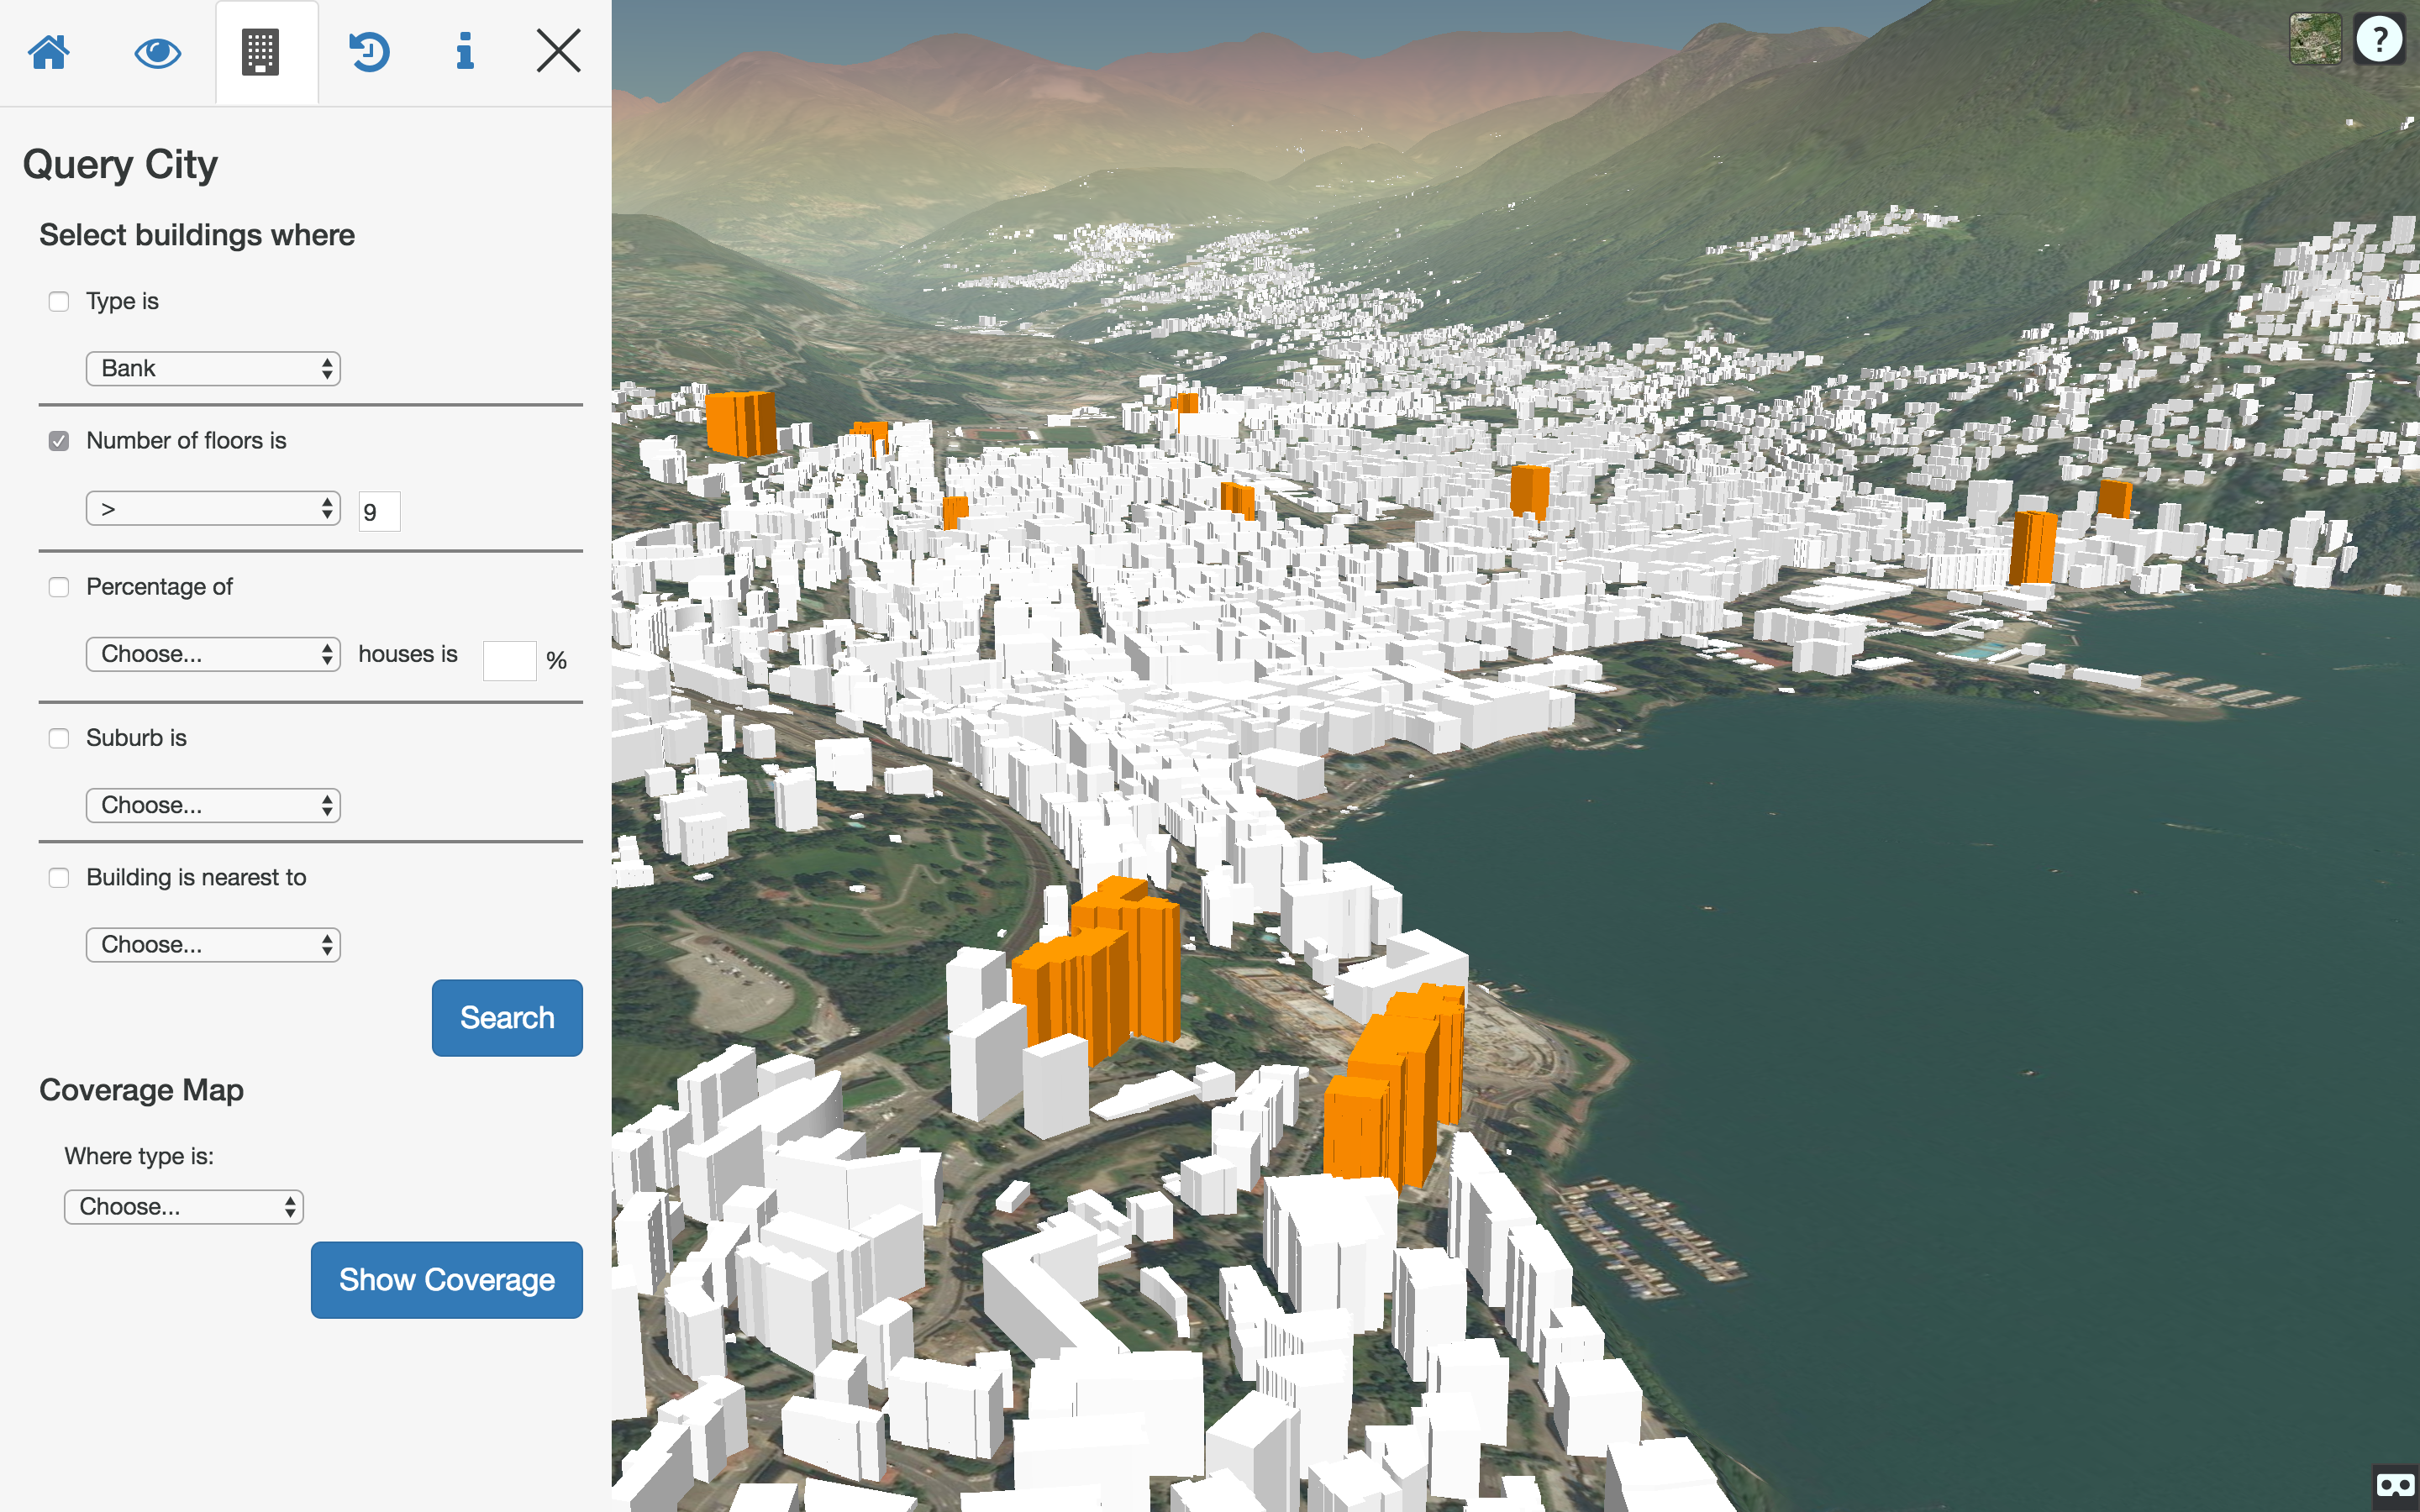
\includegraphics[width=.8\textwidth]{chapter4/images/query2}
\caption{Result of the query: ``Get all the buildings with more than 9 floors in Lugano''}
\label{fig:query2}
\end{figure} 
\begin{figure} [H]
\centering
\includegraphics[width=.8\textwidth]{chapter4/images/query3}
\caption{Result of the query: ``Get all the hospitals in Viganello (Suburb of Lugano)''}
\label{fig:query3}
\end{figure} 
\begin{figure} [H]
\centering
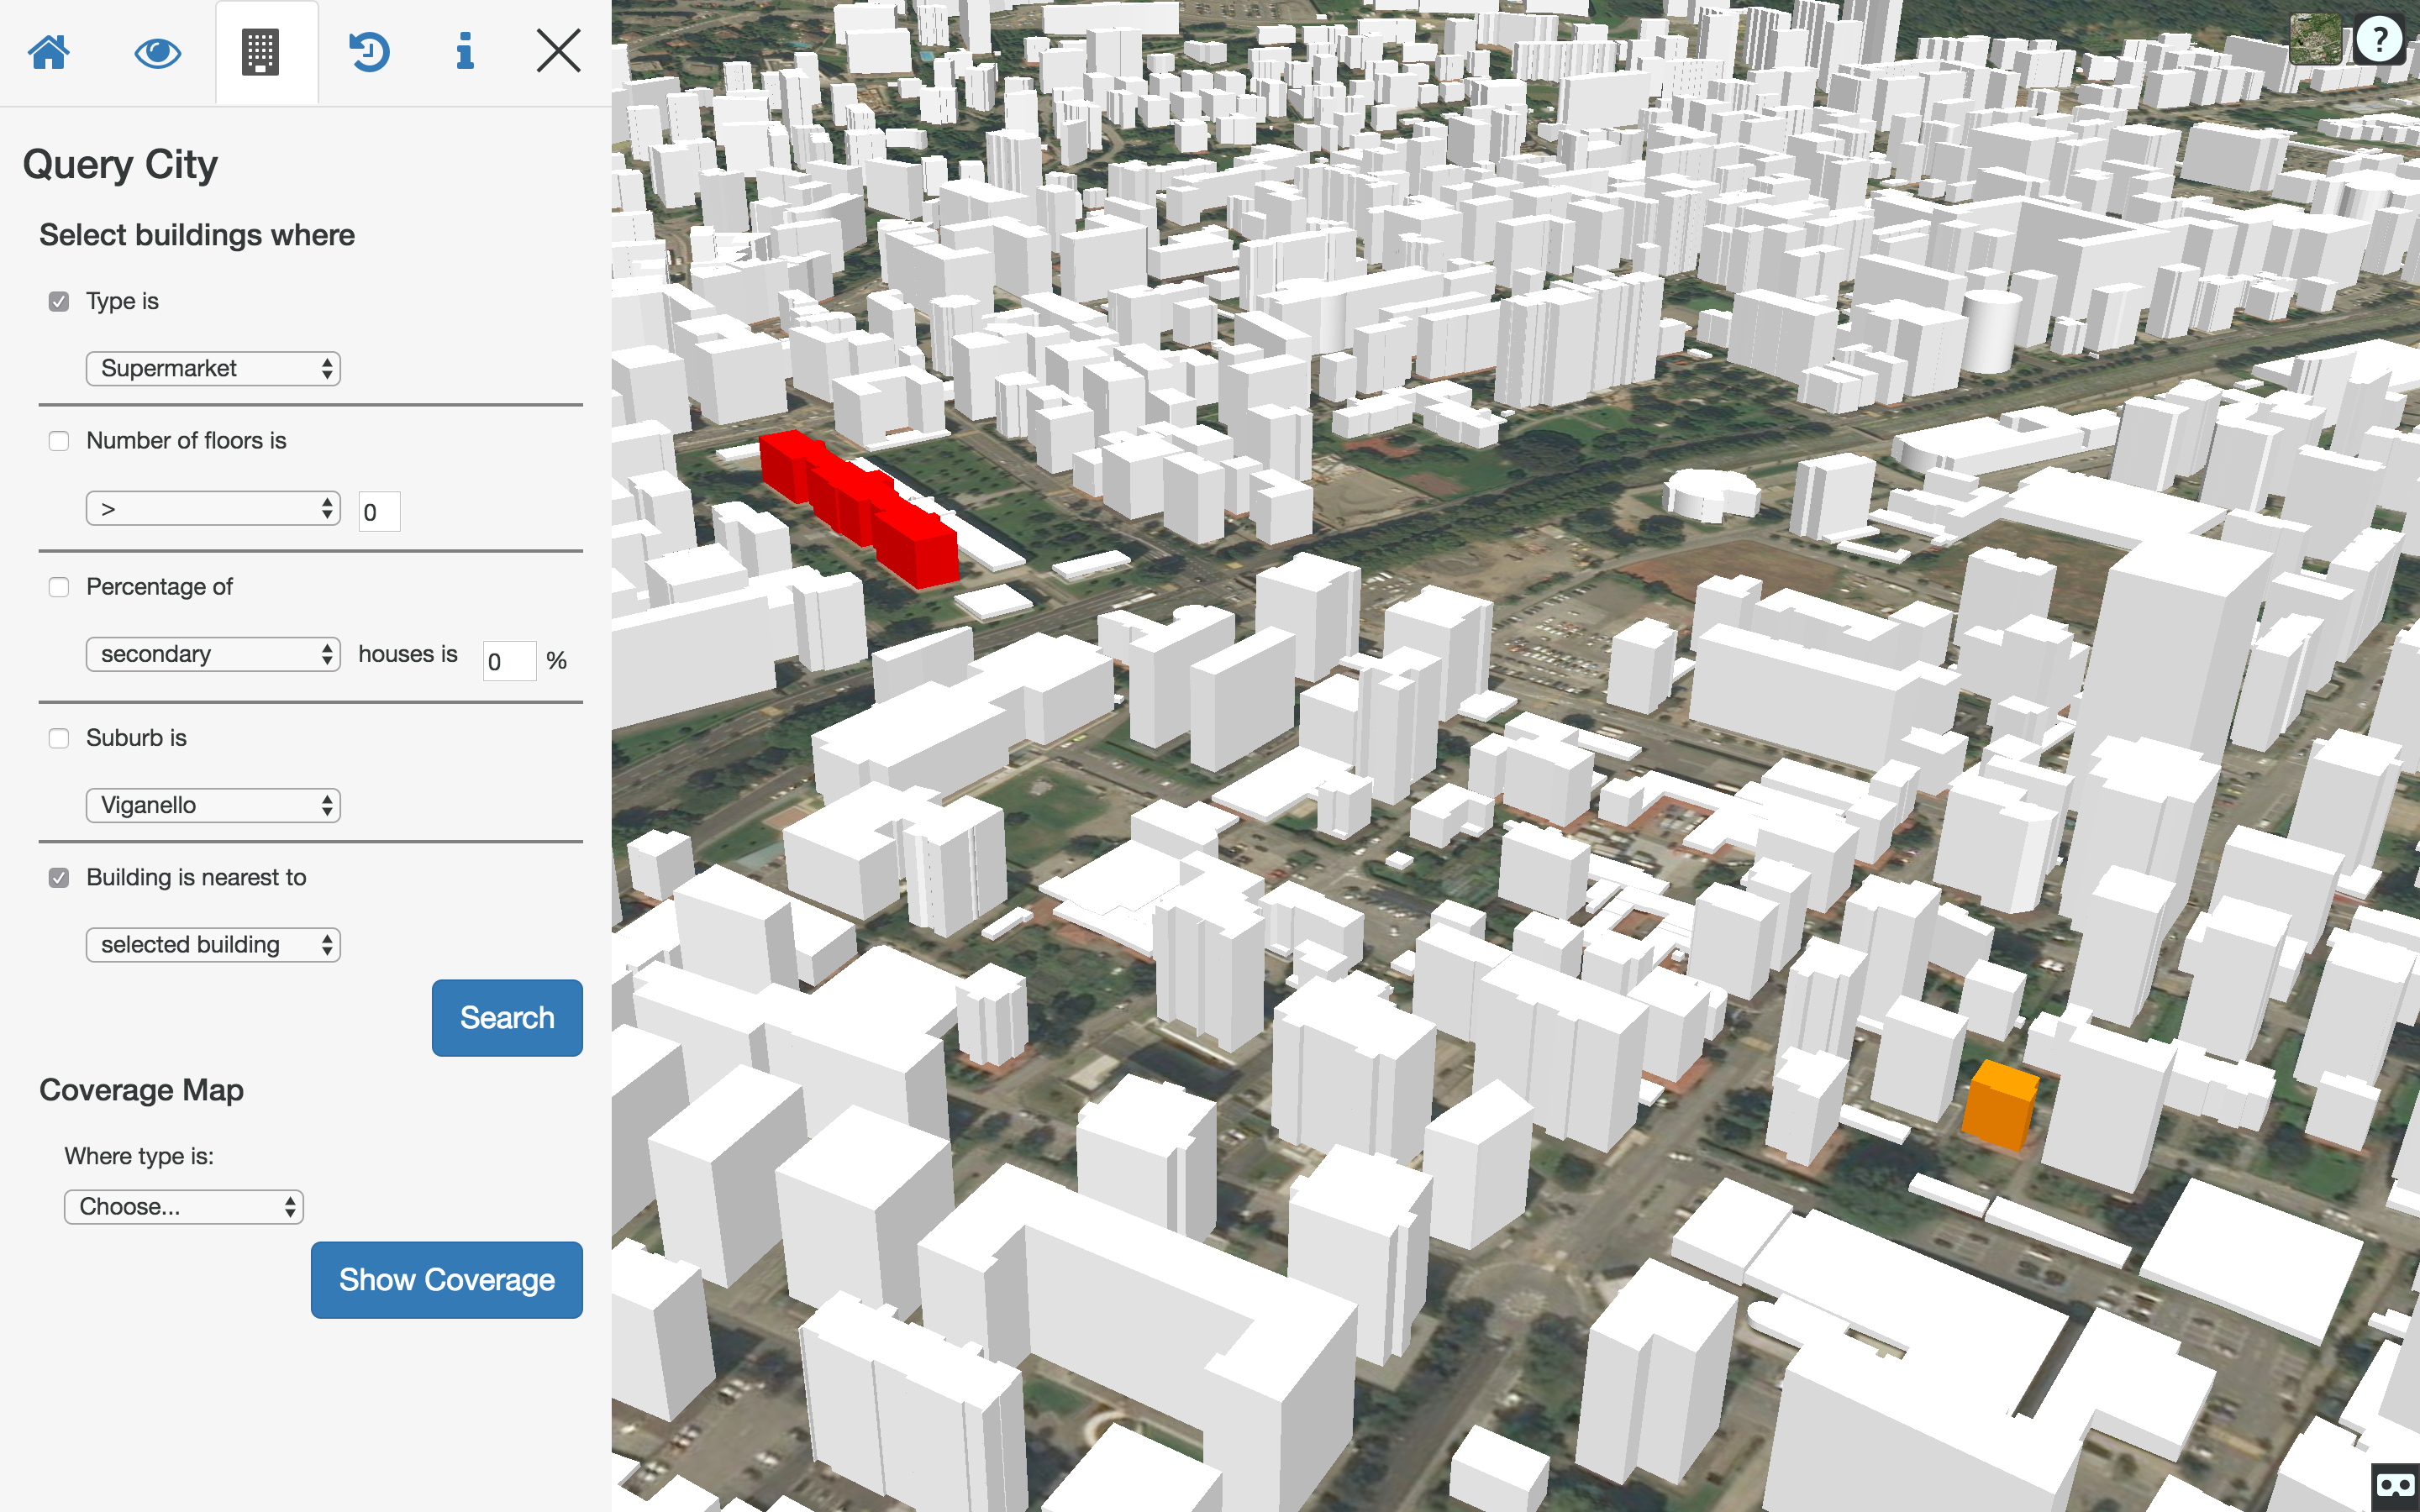
\includegraphics[width=.8\textwidth]{chapter4/images/query4}
\caption{Result of the query: ``Get nearest Supermarket near the selected building''}
\label{fig:query4}
\end{figure} 
\begin{figure} [H]
\centering
\includegraphics[width=.8\textwidth]{chapter4/images/query5}
\caption{Result of the query: ``Get all the buildings with less than 10 floors and where the percentage of primary houses is up to $70\%$ in the Suburb of Lugano''}
\label{fig:query5}
\end{figure} 

\subsubsection{City Gradient Map}

\begin{figure} [H]
\centering
\includegraphics[width=.8\textwidth]{chapter4/images/query6}
\caption{Coverage map of banks in the city of Lugano}
\label{fig:query6}
\end{figure} 
\begin{figure} [H]
\centering
\includegraphics[width=.8\textwidth]{chapter4/images/query7}
\caption{Coverage map of hospitals in the city of Lugano}
\label{fig:query7}
\end{figure} 
%%%%%%%%%%%%%%%%%%%%%%%%%
%%%%%%%%%%%%%%%%%%%%%%%%%
\section{Conclusions and future work or possible developments} \label{conclusions}
%%%%%%%%%%%%%%%%%%%%%%%%%
\subsection{Summary}
\subsection{Future Work}
%%%%%%%%%%%%%%%%%%%%%%%%%

%\begin{table}[h]
%\centering
%\scalebox {0.8} {
%\begin{normalsize}\begin{tabular}{l|lll}
%\textbf{Col 1} & \textbf{Col 2} & \textbf{Col 3} & \textbf{Col 4}\\
%\hline
%1 & 2 & 3 & Goofy\\
%4 & 5 & 6 & Mickey
%\end{tabular}
%\end{normalsize}
%}
%\caption{Caption of the table}
%\label{tab:numbers}
%\end{table}

%\cite{Stru1899a}
%%%%%
\newpage
\bibliographystyle{abbrv}
\bibliography{references}

\end{document}